\section{Introduction}


The database community has long explored new interfaces to make databases easier to access and query in various kinds of settings for both data professionals and lay users.
Typing SQL remains the main form of usage for data professionals but many lines of research have explored other new modalities: visually-oriented, touchscreen-oriented (e.g.,~\cite{10.14778/2536274.2536311}), speech-oriented (e.g.,~\cite{Shah2020}), and natural language interfaces or NLIs (e.g.,~\cite{Kim2020, gan-etal-2021-natural-sql, Scholak2021:PICARD, https://doi.org/10.48550/arxiv.2201.05966}).
In particular, a recent paper describing a SQL dictation system ~\cite{Shah2020} showed that modern automatic speech recognition (ASR) tools have matured enough to combine the benefits of dictating regular SQL in conjunction with touchscreen capabilities. Such speech-driven querying was shown to make query specification significantly faster in tablet environments, which could offer more flexibility for anywhere-anytime querying for data analysts and other data professionals.

In this paper, we go further to ask a more radical exploratory research question: \textit{If we are to design a structured query language for the speech-first era, how should it look?}
At first blush, it may sound odd to still study structured querying in the era of ChatGPT~\cite{https://doi.org/10.48550/arxiv.2005.14165, radford2018improving, openai-chatgpt-blog-post} and advances in NLIs~\cite{Kim2020}.
Why bother with anything more than mere English ``prompting''?
First off, there is a difference in motivation: NLIs mainly target lay users, while our focus is on the swathe of data professionals who are \textit{already familiar} with SQL and use it regularly. 
Second, AI models still do not offer the strong guarantee of ``correct-by-construction'' that SQL-like languages do--we know \textit{exactly what} we get in response to a query.
In contrast, AI models suffer the ``hallucination'' problem~\cite{10.1145/3571730} that can cause insidious errors that may be hard to catch, especially on arbitrary database schemas and more complex queries. 
Overall, we believe exploiting ASR to make SQL-style querying easier could supplement existing and emergent NL-to-SQL systems by contributing natural structure to an otherwise ambiguous interaction modality. To explore the validity of this belief, we designed and executed a within-subjects A/B user study to compare the ease of use of a new speech-first dialect of SQL, SpeakQL, against SQL. We exclude ChatGPT and other AI models from our study because we are interested in the ease of use of a \textit{structured} query language, not a natural language interface.

%Add statement on how chat GPT is not part of our problem statement here. Saying we think this can help data professionals is probably too strong of a statement. Couch this more as a question of how to make SQL easier to use for data professionals.


\begin{figure}[t]
  \centering
  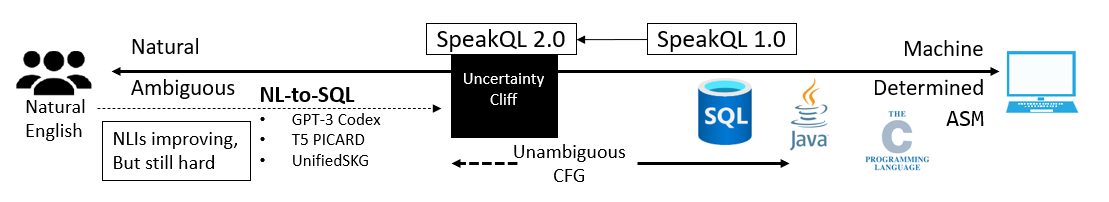
\includegraphics[width=\linewidth]{figures/naturalness and languages.png}
  \caption{Bridging the gap between naturalness and determinism in programming languages; extension of figure from~\cite{Shah2020}.}
  \label{fig:cliffdiagram}
\end{figure}


\paragraph{\textbf{Desiderata}} 
We start by describing some desirable properties of a spoken structured query language motivated by balancing \textit{usability for specification} and \textit{practicality in design}.
(1) Minimal deviation from SQL to ensure it is easy to pick up for people who know SQL already. 
(2) Less rigid than SQL and more natural English-style flow in structure for the speech modality. 
(3) Unambiguous context free grammar (CFG) to ensure a valid spoken query can be translated to a \textit{semantically equivalent} SQL query to enable use of an RDBMS as is for query execution.
% objective is to design a dialect of SQL that improves user experiences when using speech to interact with databases and that can be integrated into a speech-driven query system. 



\paragraph{\textbf{Our Approach}}
In this paper, we explore the potential benefits of natural syntax by designing and evaluating a \textit{new dialect of SQL} for spoken querying in response to the above desiderata. We call our dialect SpeakQL 2.0 or just \textit{the SpeakQL dialect}.
Figure~\ref{fig:cliffdiagram} illustrates where SpeakQL 2.0 falls in the spectrum of naturalness and determinism. 
Unlike NLIs that do not offer correctness guarantees, SpeakQL 2.0 has an unambiguous CFG. 
But it is less rigid than regular SQL although it is not multimodal (no touchscreen component) like what SpeakQL 1.0 proposed~\cite{Shah2020}.
We design the SpeakQL dialect as an extension of the ANSI SQL grammar. 
It has several features to help increase the ``naturalness'' of speaking queries in the style of ``stream of thought'' instead of specifying everything all at once.

\eat{
 SpeakQL dialect features are defined in a modified Backus-Nair form (BNF) which is built from a publically available MySQL grammar. SpeakQL queries are parsed with an Antlr-based Java application and translated via AST (abstract syntax tree) manipulation using a Python-based program that performs operations on an AST class representative of the parsed query. 
}

\paragraph{\textbf{Motivating Applications}}
Before explaining the dialect's features, we describe some motivating application scenarios for spoken structured querying with a dialect such as SpeakQL.

\begin{itemize}

\item \textit{On-the-go ad hoc database access.}
Data-driven operations are now common in many domains. 
Organizations with field-based assets who operate in remote or austere environments such as the military~\cite{armydatascientists} and the oil-and-gas industry~\cite{MOHAMMADPOOR2020321} may face barriers to purely typing-based or touch-based data access on the field. 
Such barriers could be due to lack of workspace for keyboards, personal protective equipment requirements impeding typing/touching, or on-the-go working conditions such as a mobile headquarters. 
Spoken querying boosts capabilities in such settings for on-the-go ad hoc database access. 
As an example, suppose a military cyber-defense team in the field that must wear protective equipment detects anomalous behavior on some client devices. 
Pre-built (canned) analytics dashboards may not address all their unexpected querying needs. 
NLIs run the risk of erroneous query translation. 
But dictating a precise structured query can empower the team to access and analyze relevant network traffic data without compromising team security, agility, and query fidelity.

\vspace{2mm}
\item \textit{Assistive technology for people with motor impairment.} 
The U.S.~Bureau of Labor Statistics data shows that in 2020 in the IT and engineering sectors, 18\% of nonfatal injuries/illness involving days away from work were in the upper extremities, viz., shoulders, arms, hands and wrists~\cite{blsinjurydata2020}. For such people, as well as for many people with arm disabilities, typing, clicking, or touchscreens may not be viable as a modality but speech can be a powerful modality.
Thus, spoken structured querying can help data professionals with such disabilities or injuries.

\eat{
\subsubsection{Guaranteed Correctness from Natural Expressions}
Natural language (NL) models have seen a recent rapid advance in capability and it is logical for a speech-enabled query dictation system to employ one of several capable NL-to-SQL systems \cite{https://doi.org/10.48550/arxiv.2005.14165, Scholak2021:PICARD, https://doi.org/10.48550/arxiv.2201.05966}. However, while large language models have vastly improved NL-to-SQL accuracy over previous attempts, ambiguities inherent in natural language present an AI-hard problem: eliminating all uncertainty from the result of an NL-to-SQL translation result. Because NL-to-SQL accuracy is not perfect, users must validate query correctness after the model generates SQL code. We seek to overcome this obstacle at the point of query dictation (see Figure \ref{fig:cliffdiagram}) rather than result generation.
}

\end{itemize}

\paragraph{\textbf{User Study-based Evaluation}}

In this paper, we focus primarily on evaluating the \textit{usability} of the SpeakQL dialect's features designed for spoken querying compared to regular SQL. 
We leave more extensive comparisons with other querying modalities or integration with multimodal interfaces to future work.
We implemented the SpeakQL dialect and conducted a within-subjects A/B user study. 
We had 22 participants, all students familiar with SQL and relational databases. 
They were given a 6-table university database schema and asked to speak 12 queries, half designed to be simple and half, complex. The user study was conducted over a span of 4 months. 
Performance was measured in terms of both the time required to plan and specify a full query in response to an English prompt posed and the number of attempts till a fully correct query.

Overall, we find no statistically significant differences in the total query specification time for SQL vs. the SpeakQL dialect. 
This suggests that SpeakQL's extra verbosity was compensated for by lower thinking effort/time.
Indeed, on average SpeakQL sees slightly lower median specification times for planning the complex queries. 
We also find that participants get better at speaking SpeakQL as they become more familiar with its features. 
The mass of qualitative textual feedback from the post-participation surveys also offer numerous interesting insights into the strengths and current weaknesses of SpeakQL. 
We see both positive and negative feedback on both the dialect and its individual features.
But in aggregate, participants reported that SpeakQL made it ``much easier'' or ``somewhat easier'' to use than SQL between half to four-fifths of the time depending on the feature. 
Natural functions and unbundled queries were the most highly liked and used features, while synonyms were (perhaps surprisingly) deemed not that useful. 
In all, our user study results and surveys suggest that the SpeakQL dialect is indeed user-friendly. 
We hope it spurs more research conversations in the community on more design iterations, additional features, and ultimately, fully fledged spoken querying for databases in more contexts.

\paragraph{\textbf{SpeakQL Design and Features.}}
The SpeakQL dialect has 4 new features with increasing sophistication, grouped into 2 categories: smaller local changes to the grammar's production rules and deeper structural changes with more complex rules. 
Each feature is \textit{optional}, which means regular SQL syntax is also valid in SpeakQL. 
Section 3 dives into their details with examples but we summarize their rationale here. 
The first category has the following two features. 
(1) \textit{English synonyms} for some SQL keywords such as SELECT and FROM. 
(2) \textit{Natural functions} to omit speaking of special character symbols such as commas and parentheses in some contexts.
These two extensions make SpeakQL sound less like code and more like English (compared to SQL). So, they enhance the ``naturalness'' of the spoken query.

The second category has the following two features. 
(3) \textit{Clause reordering}. Specifically, the SELECT, FROM, and WHERE clauses can be spoken in any order. Query modifier clauses such as GROUP BY and ORDER BY too can be reordered. 
(4) \textit{Unbundling} of complex queries into per-table decomposed queries. 
This allows users to reason about one table at a time instead of ``all at once'' like in SQL. 
This is inspired by function-stitching style programming seen for Python Pandas and Spark DataFrame. 
It can reduce the amount of schema context to keep in mind when speaking, albeit at the cost of raising verbosity and query token lengths. 
Overall, these two features reduce query rigidity and offer more freedom for ``stream of thought'' querying.

\eat{
Keyword synonyms expand the available vocabulary for select expressions and allow users to select specific types of keywords depending upon the nature of their query. Additionally, synonyms that represent symbols (e.g. replacing a comma with the word \emph{and}) improve naturalness by reducing the amount of symbols that must be verbalized. Optional ordering relaxes the rigid structure of the typical SQL SELECT, FROM, WHERE expression, allowing users to reason about queries in different orders based on preference and query type. The optional ordering feature also extends to additional expressions such as GROUP BY, \emph{order by}, HAVING, and \emph{limit}. Symbol dictation is further reduced with the natural functions feature, enabling the expression of aggregator functions without parentheses. Finally, the unbundling feature breaks complex queries into smaller single-table query parts and allows users to reason about query formulation one table at a time.
}


\vspace{2mm}
To summarize, this paper makes the following technical contributions:

\begin{packeditems}

\item To the best of our knowledge, this is the first paper to systematically study and evaluate an extension to SQL tailored for spoken querying. 

\item We present the SpeakQL dialect with four new features that raise naturalness and reduce rigidity compared to SQL, while preserving correct-by-construction guarantees with a context free grammar.

\item We describe the implementation of the SpeakQL dialect, including its grammar rules and our translator to convert any SpeakQL query to regular SQL to ensure it can be used for existing RDBMSs.

\item We present an extensive user study-based evaluation of SpeakQL vs. SQL for spoken querying. Our empirical findings, both quantitative and qualitative, suggest the usability of such a dialect and also offer avenues for more research to improve it.

\end{packeditems}




\section{Background}


\subsection{The Structured Query Language (SQL)}

\paragraph{\textbf{Origins and Purpose}}

Introduced in 1974~\cite{Chamberlin1974}, SQL is nearing its 50th birthday. Despite (or perhaps because of) its age, it remains the de facto standard language for database quyering. SQL (originally named SEQUEL) was intended for both application programmers and a non-programmer target audience of business professionals and other laypersons requiring data access from relational databases~\cite{Chamberlin1976}. Its initial design and following updates were informed by a user-centric approach, and it is perhaps one of the first programming languages for which human-computer interaction considerations were deliberately studied~\cite{Reisner1975,Reisner1977}. Due to its high popularity, declarative nature, targeted purpose, structured syntax, and human-centric design, SQL is a natural starting point for a spoken query language.

\paragraph{\textbf{Syntax Grammar and SQL Variants}}

All SQL grammars include syntax rules for both \emph{data definition language} (DDL) and \emph{data manipulation language} (DML) statements. DDL statements are intended to enable specification of data structure; and DML statements enable data access and update functions \cite{DBLP:books/aw/AbiteboulHV95}. Data analysts, informaticists, and other data consumers generally make use of DML statements to fulfill data requirements. DDL statements are generally expressed by database administrators and software developers responsible for designing, implementing, and maintaining data models within database management systems. 

Numerous variants of SQL syntax exist from multiple vendors and open source projects. While each variant tends to contain implementation-specific features targeted at specific RDBMSs, most (if not all) generally adhere to the ISO/IEC 9075-1:2016 information technology standard for SQL~\cite{kelechava_2020}. Seven SQL grammars are available under various open source licenses on the ANTLR parser Github repository including: Hive, MySQL, PL-SQL, PostgreSQL, SQLite, Trino, and T-SQL~\cite{antlrgrammarsv4}.


\paragraph{\textbf{Human Factors}}
Human factors evaluations were conducted as part of the SEQUEL development effort. Usability experiments comprised of teaching SEQUEL to programmer and non-programmer college students. The study yielded several results, including the recommendation to make SEQUEL a layered system consisting of three layers representing increasing levels of complexity, and the recommendation to replace complicated correlation and computed variable syntax with the join feature, which most SQL users are familiar with now.

Reisner also discovered that sources of minor errors when converting English statements into SEQUEL queries included ending errors, spelling errors, and synonym errors. These discoveries resulted in the recommendation to incorporate spelling correction, introduce a synonym dictionary to the language syntax, and a create stem-matching procedure as user aids that would enable users to use keywords with various forms of conjugation.~\cite{Reisner1977} In a later study, Reisner also confirmed that query complexity has a directly proportional effect on the likelihood of error occurrence during query formulation~\cite{Reisner1975}.

A more recent SQL usability study revealed that user tendency toward invalid syntax synonyms, omission of punctuation, and the NL-like nature of some SQL keywords can be sources of programming errors among novice users. Table joins, aliases, and subqueries were also identified as significant sources of programming errors~\cite{10.1145/3514214}.

\subsection{Natural and Controlled Natural Languages}

\paragraph{Natural Language Interfaces}

Natural language interfaces (NLIs), such as the recently popular ChatGPT~\cite{radford2018improving, https://doi.org/10.48550/arxiv.2005.14165, openai-chatgpt-blog-post}, show that NL-based chatbots can be a viable tool for many purposes, including NL-to-SQL querying, wherein users express their query intent in regular English. NL-to-SQL is still an active area of research~\cite{Kim2020, https://doi.org/10.48550/arxiv.2005.14165, Scholak2021:PICARD, https://doi.org/10.48550/arxiv.2201.05966, 10.1145/3318464.3383128}, and it has strong potential to lower the barrier to entry to lay users (people without SQL knowledge).
But NLIs still suffer from three issues in technical applications such as database querying that data professionals may be wary of: \textit{ambiguities}, which can confound user goals; \textit{out-of-vocabulary terms}, common in database schemas and predicate content, can hinder accurate translation; and \textit{lack of correctness guarantees}, compounded by the ``hallucination'' problem of generative NLP models. Additionally, users may tend to seek out a \emph{latent syntax} when performing coding tasks with a NL interface to ground their uncertainty about language model capabilities~\cite{10.1145/3491102.3501870}.
That said, recent research suggests that NLI with more restricted grammar and/or structure can improve user experience for technically complex tasks~\cite{mu2019do}.

\paragraph{Controlled Natural Languages}

Controlled or restricted NL are based on an NL such as English but more restrictive in their lexicon, syntax, and semantics. 
They retain a majority of its base NL properties and are defined explicitly~\cite{10.1162/COLI_a_00168}. 
Most PLs (including SQL) are not controlled NLs because their syntax deviates too much from the NL and have many statements that do not exist in the NL. 
Controlled NLs have been evaluated against linear keyword languages such as SQL and found to be easier for novice users for performing data retrieval tasks~\cite{doi:10.1287/isre.3.3.252}. Early research on controlled query languages suggests a continuum between formal and natural language exists with a mid-point serving as an optimal combination of structure and flexibility~\cite{10.1145/800045.801602}.
In contrast to NL-to-SQL described previously, a controlled NL does offer the benefit of being ``correct-by-construction'' at the cost of being less flexible than a natural language interface.

\paragraph{Naturalness}

Naturalness of a controlled NL can be evaluated by how close an expression in it is to its base NL. 
This is evaluated in terms of both \emph{readability} and \emph{understandability}. 
These criteria can range from completely unnatural, where the controlled NL uses symbols, characters, and unnatural keywords, to languages with natural sentences where the controlled NL can yield expressions that appear as if they were written in the base languages~\cite{10.1162/COLI_a_00168}.

\subsection{SpeakQL}

Prior work on SpeakQL 1.0, a speech+touch multimodal querying interface ~\cite{Shah2020}, was aimed at data professionals such as data analysts, nurse informaticists, and DBAs who desired ad-hoc on-the-go querying in settings without a regular computer but with mobile devices such as a tablet. 
That paper's user study showed that the SpeakQL interface reduced query specification times vs.~typing SQL in such settings by 2.7x on average. 
But conversations with such data professionals in that work revealed a key functionality gap: 
people with SQL knowledge may want to do a quick record retrieval or analytics query in an ad-hoc setting where even touchscreens are unviable for query specification, let alone keyboards, but voice is feasible. 
Speech-driven querying can also help people with disabilities or temporary injuries and perhaps also augment conversational assistants such as Alexa, Siri, etc. to aid in database querying. 
That provided the basis for this exploratory work on a spoken SQL dialect. 



\section{Our SpeakQL Dialect}


We now present our prototype speech-first dialect extension of SQL. 
We overload the prior art interface name to call our dialect SpeakQL.  
It has four new features, all optional for usage:

\begin{itemize}
  \item Keyword Synonyms and Optional Syntax
  \item Natural Functions
  \item Query Clause Ordering
  \item Complex Query Unbundling
\end{itemize}

SpeakQL can be considered a controlled NL based on English that extends SQL. Note that SQL is a constructed language rather than a controlled NL. This distinction arises because the objective of the SpeakQL dialect is to increase naturalness of specifying queries, achieved via the introduction of English grammar features and the reduction of special character (non-alphabet) symbol usage in SpeakQL queries. 

We defined the SpeakQL grammar by extending a big part of the MySQL grammar from the Antlr4 repository~\cite{antlrgrammarsv4}. We added additional production rules within existing SQL rules to realize our features. This means that SpeakQL is a \textit{superset} of that chosen SQL subset. That is, a query constructed using the regular SQL syntax and keywords is a valid SpeakQL query too. So, users can ``fall back'' on regular SQL if they desire to.

\subsection{Keyword Synonyms and Optional Syntax}

This is a simple feature designed to increase the naturalness of an SQL query by enabling more sentence-like expressions. The intuition driving the development of these features is that speech patterns may be more amenable to use NL-like behavior, e.g., omitting syntax such as symbols and punctuation but including concepts such as determinatives (e.g., THE) and prepositions (e.g., OF).

\subsubsection{\textbf{Synonyms}} 
This feature is motivated in-part by early human-computer interface research performed on SQL users~\cite{Reisner1977} that recognized the benefit of syntax synonyms and optional word stemming, as well as more recent observations on tendencies toward synonyms~\cite{10.1145/3514214}.
We introduce SQL keyword-equivalent synonyms for the most common DML syntax keywords: SELECT, FROM, and JOIN, as well as for the comma as a column- or table-delimiter within the SELECT and FROM clauses, respectively. 

\begin{table}
  \centering
  \caption{Synonyms in SpeakQL for SQL keywords.}
  \begin{tabular}{|m{6em} m{18em}|}
    \hline
    \textbf{SQL Keyword} & \textbf{SpeakQL Synonyms} \\
    \hline
    SELECT & Select, Find, Retrieve, Get, Show Me, Display, Present, What Is, What Is The, What Are, What Are The \\
    \hline
    FROM & From, From table, From Tables, In Table, In Tables \\
    \hline
    ' , ' (Comma) & ' , ' (Comma), And \\
    \hline
    JOIN & Join, Join Table, Join With Table, By Joining, By Joining Table, By Joining With Table, Joined With, Joined With Table \\
    \hline
  \end{tabular}
  \label{tab:keyword-synonyms}
\end{table}

Keyword synonyms are listed in Figure \ref{fig:synonymsslide}.

\begin{figure*}
\centering
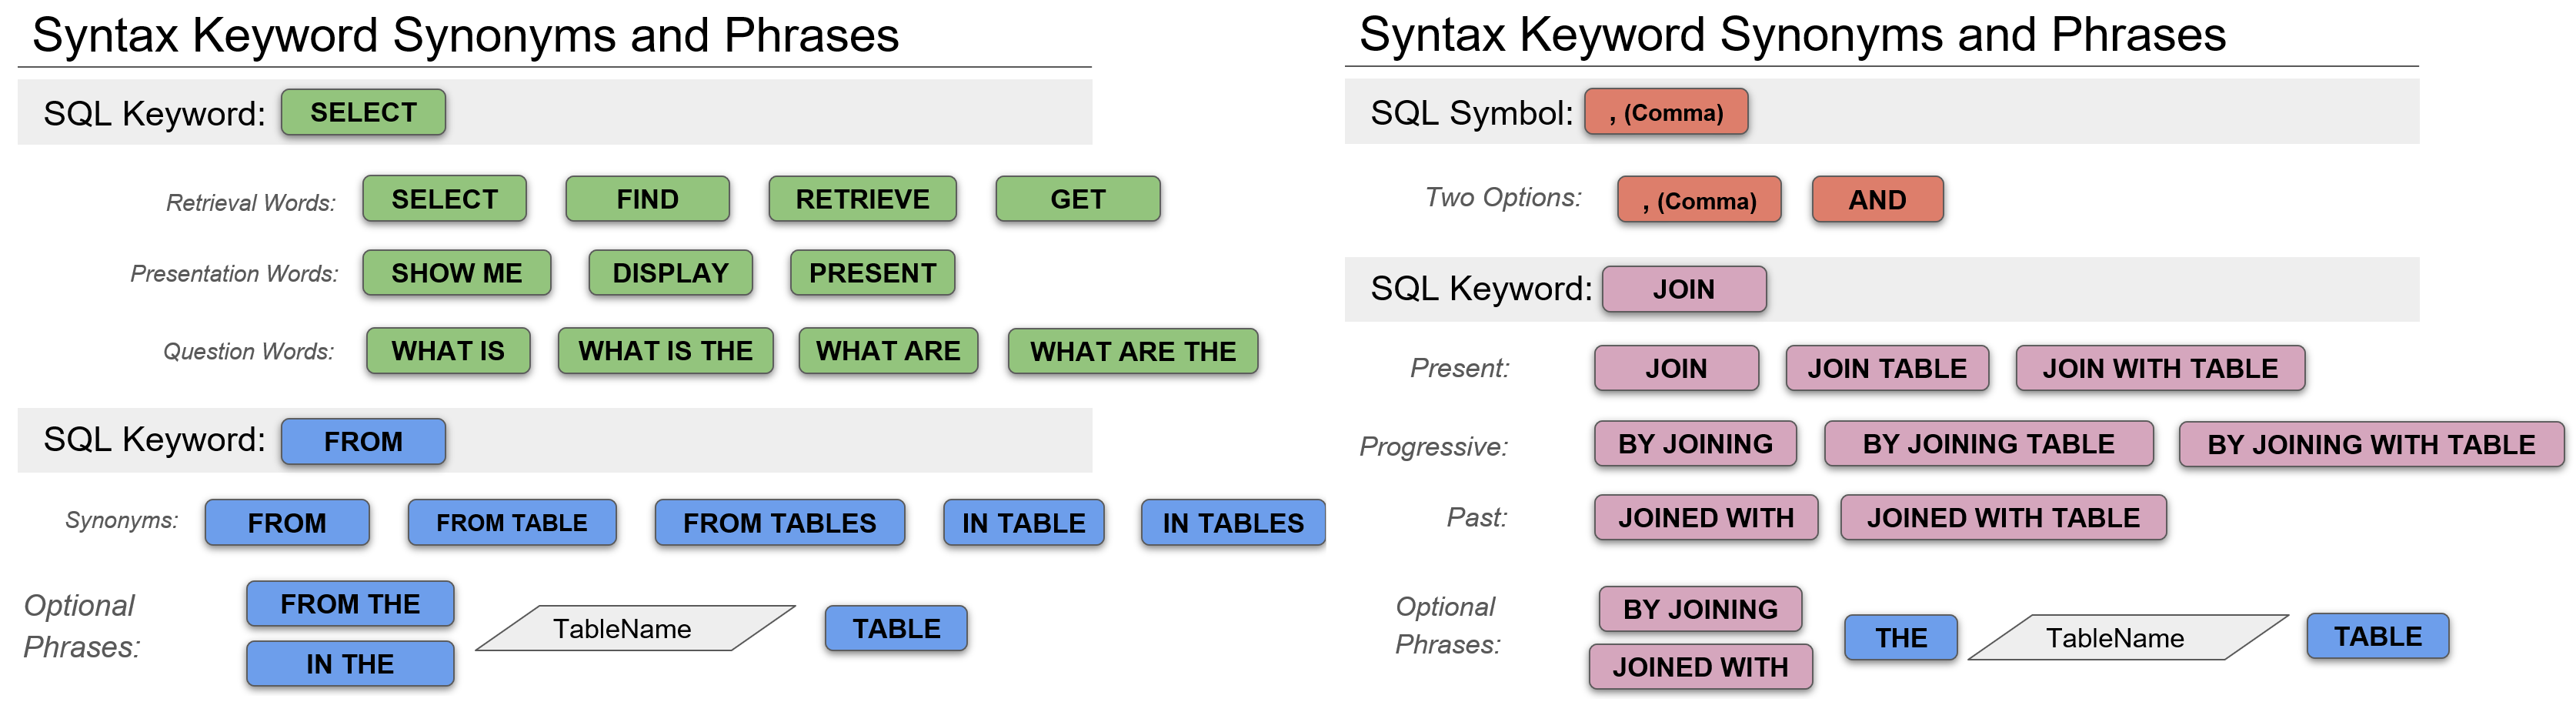
\includegraphics[width=\textwidth]{figures/all_synonyms.png}
\caption{SpeakQL Synonyms}
\label{fig:synonymsslide}
\end{figure*}

\subsubsection{\textbf{Optional Syntax}} 
SpeakQL allows for the use of optional THE and TABLE keywords when dictating a table expression. 
This permits expressions such as \emph{SELECT everything FROM THE courseoffering TABLE}, which can be more natural for speaking than the SQL equivalent \emph{SELECT everything FROM courseoffering}. 
Introducing the THE keyword as a determinant clarifies the context of the subject of the SpeakQL sentence, which is the \emph{courseoffering} table. 
Appending the TABLE keyword to the expression provides further context and clarity that the referenced table is a tangible object within the database. While neither keyword changes the expression's meaning, their usage improves the naturalness of the SELECT statement, thus potentially improving the dictation experience.


\subsubsection{\textbf{Examples}}

%Example query
\begin{verbatim}
  SQL: SELECT area, wheelchairspaces 
       FROM room WHERE floor = 2;
\end{verbatim}
\paragraph{SpeakQL} \emph{\textbf{Show me} area and wheelchairspaces \textbf{in the} room \textbf{table} where floor equals 2}

\vspace{2mm}
%Example query
\begin{verbatim}
  SQL: SELECT COUNT(id) FROM course;
\end{verbatim}
\paragraph{SpeakQL:} \emph{\textbf{What is the} count parenthesis id parenthesis \textbf{in the} course table}



\subsection{Natural Functions}

\begin{figure*}[ht]
    \centering
    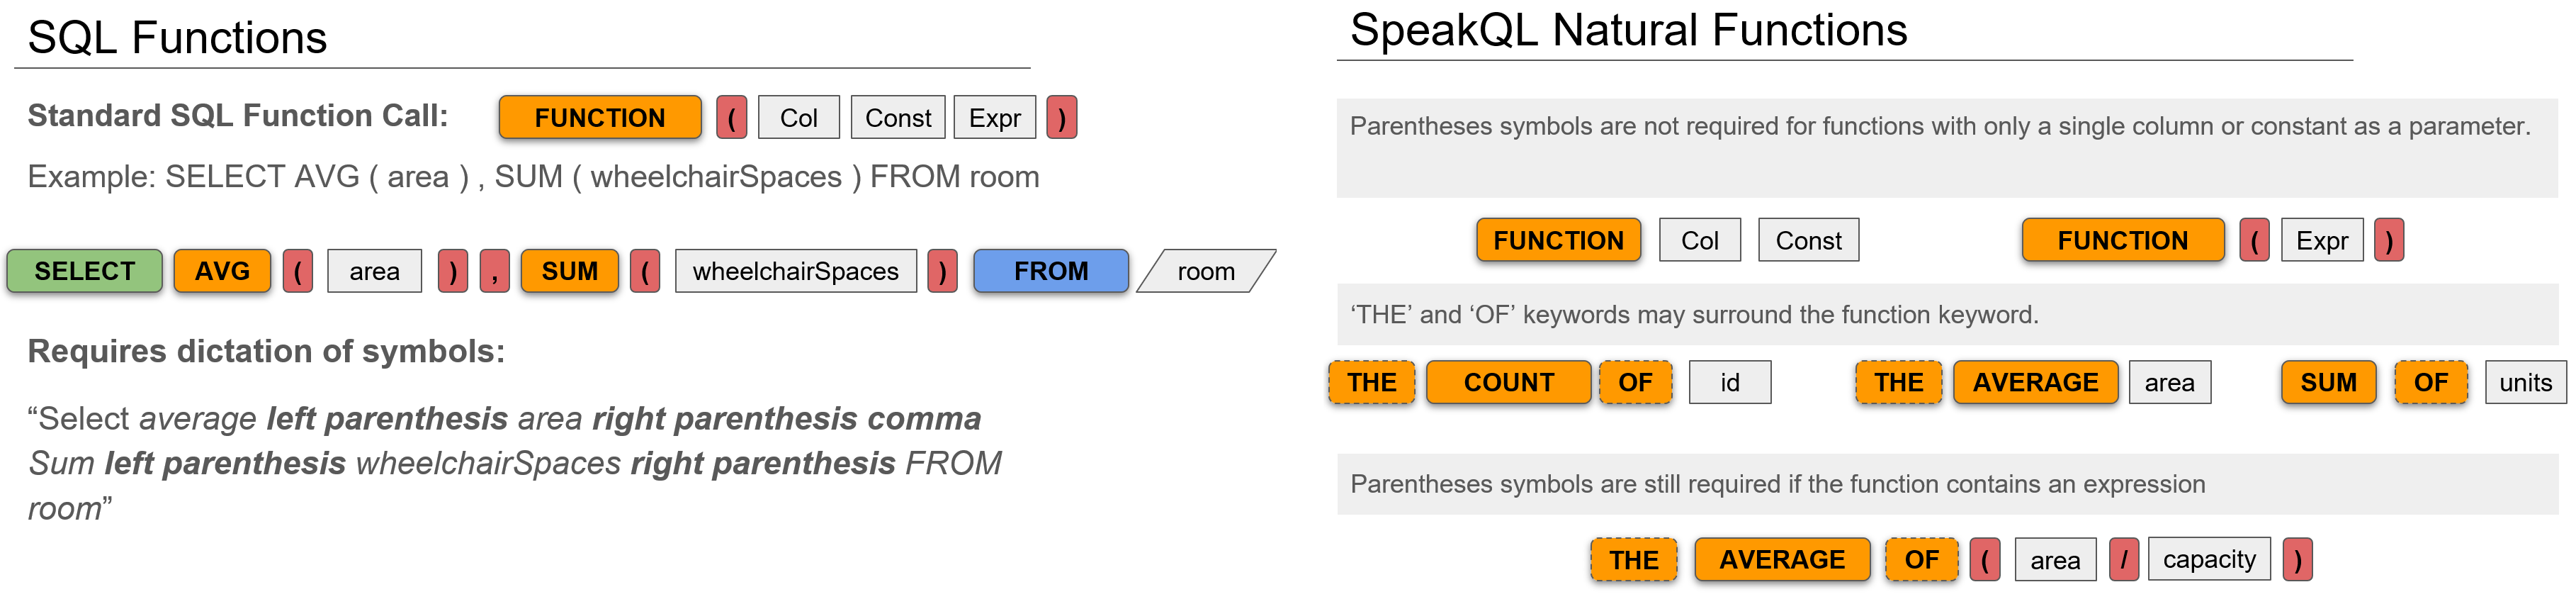
\includegraphics[width=\textwidth]{figures/natural_functions.png}
    \caption{Natural Functions}
    \label{fig:naturalfunctions}
\end{figure*}

The SQL subset we support includes aggregator functions such as SUM, AVG, and COUNT. 
In the prior work on the SpeakQL interface, users had to verbalize the parentheses symbols, which reduces the naturalness of dictation. 
While parentheses are often essential for disambiguation, for the SpeakQL dialect we identified a set of function references in which parentheses could be omitted safely without affecting the query's semantic meaning. 
Specifically, our SpeakQL dialect permits the expression of functions naturally, that is without verbalizing parenthesis, for functions that have a single constant or column as an argument. 
This feature also permits the optional syntax keywords THE and OF to surround the function name, resulting in more NL-like sentence expressions. 

However, if the query intent involves the inclusion of an expression as a function argument, the verbalization of parenthesis remains a requirement. This allows the SpeakQL dialect to retain SQL's capability to pass mathematical, comparative, and subquery expressions as function arguments within the boundaries of dictated parentheses, ensuring we avoid ambiguity such as cases in which neighboring SELECT clause elements get misinterpreted as function arguments by the translator.

Natural function syntax and examples are portrayed in Figure \ref{fig:naturalfunctions}.


\subsubsection{\textbf{Examples}}

%Example query
\begin{verbatim}
  SQL: SELECT COUNT(id) FROM course;
\end{verbatim}
\paragraph{SpeakQL} \emph{\textbf{Get the count of} id \textbf{from the} course  \textbf{table}}

\vspace{2mm}
%Example query
\begin{verbatim}
  SQL: SELECT AVG(units), COUNT(title)
       FROM course
\end{verbatim}
\paragraph{SpeakQL:} \emph{\textbf{Find the average} units \textbf{and the count of} title \textbf{in the} course \textbf{table}}



\subsection{Query Clause Ordering}

\begin{figure}[H]
  \centering
  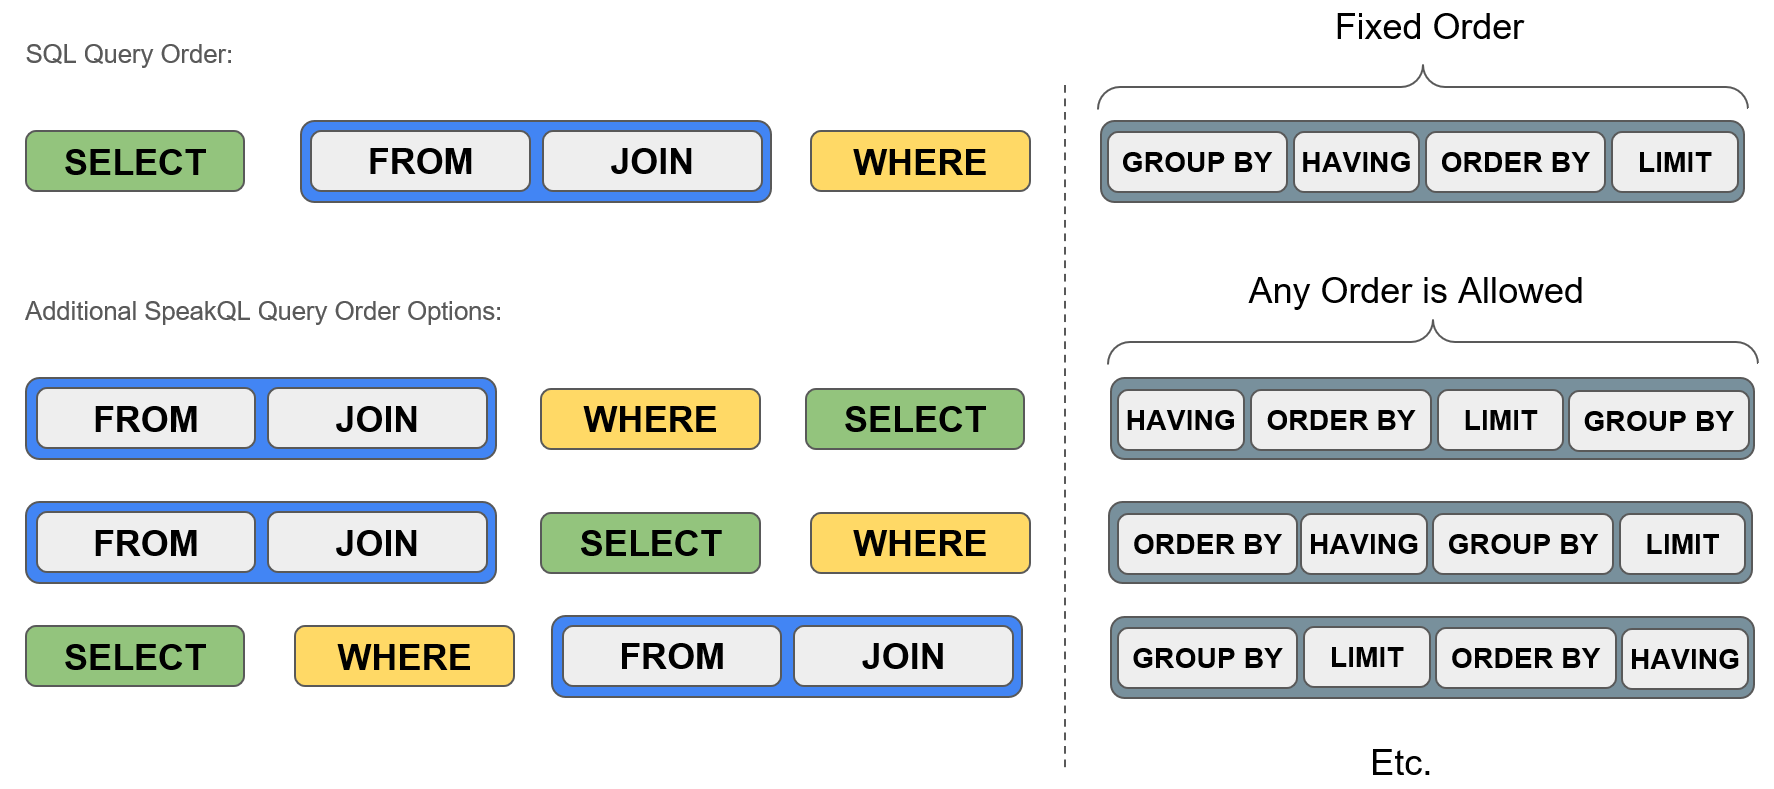
\includegraphics[width=0.6\linewidth]{figures/alternate_ordering.png}
  \caption{Alternate Ordering}
  \label{fig:alternate_ordering}
\end{figure}

This feature allows for optionally reordering the SELECT, FROM/JOIN, and WHERE clauses, as well as the GROUP BY, HAVING, ORDER BY, and LIMIT clauses. 
That is, these clauses may appear in any order within a SpeakQL statement. 

\subsubsection{\textbf{SELECT-FROM-WHERE Ordering}} 
Intuitively, we recognize that there are alternate paths to forming a SQL query. In some instances, the SELECT, FROM, WHERE ordering of SQL syntax is the order a user may find most-useful when dictating a query. In other cases, users may wish to reason about table sources and joins prior to defining columns and functions; alternatively, users may wish to establish restrictions using where predicates before defining other aspects of a query. Additionally, alternate ordering provides "second chances" for query recovery. For example, if a user is dictating a query and defines the SELECT and WHERE clauses, forgetting to state the table source, they may resolve this omission by dictating the FROM clause at the end of the query rather than starting over from the beginning.

\subsubsection{\textbf{Modifier Ordering}} 
The \emph{modifier}  optional ordering feature (in this paper modifiers refer to the GROUP BY, HAVING, ORDER BY, and LIMIT expressions) is partially motivated by the observation that queries that require multiple modifier statements such as GROUP BY and HAVING tend to be more complex than simple single table queries or queries with a single modifier such as GROUP BY \cite{10.1145/2729094.2742620}. SQL syntax requires that these clauses occur in the strict order GROUP BY, HAVING, ORDER BY, and LIMIT. If these clauses appear out of order within a query, it is invalid and requires correction. While this is not a significant problem for typed queries, as they can easily be rearranged in a text editor, if such an error is introduced during the spoken querying process, more sophisticaed error correction is required and the query speaker must likely re-dictate the entire query.




\subsubsection{\textbf{Examples}}

%Example query
\begin{verbatim}
  SQL: SELECT DISTINCT termperiod FROM term 
       WHERE year = 2022;
\end{verbatim}
\paragraph{SpeakQL} \emph{\textbf{From} \textbf{the} term \textbf{table show me distinct} termperiod  \textbf{where} year equals 2022}

\vspace{2mm}
%Example query
\begin{verbatim}
  SQL: SELECT facultyname, ondays 
       FROM courseoffering 
       WHERE capacity > 20 
       ORDER BY facultyname LIMIT 10;
\end{verbatim}
\paragraph{SpeakQL:} \emph{\textbf{In the} courseoffering \textbf{table where} capacity is greater than 20 \textbf{find} facultyname \textbf{and} ondays \textbf{limit} 10 \textbf{order by} facultyname}


\subsection{Query Unbundling}

\begin{figure}[ht]
  \centering
  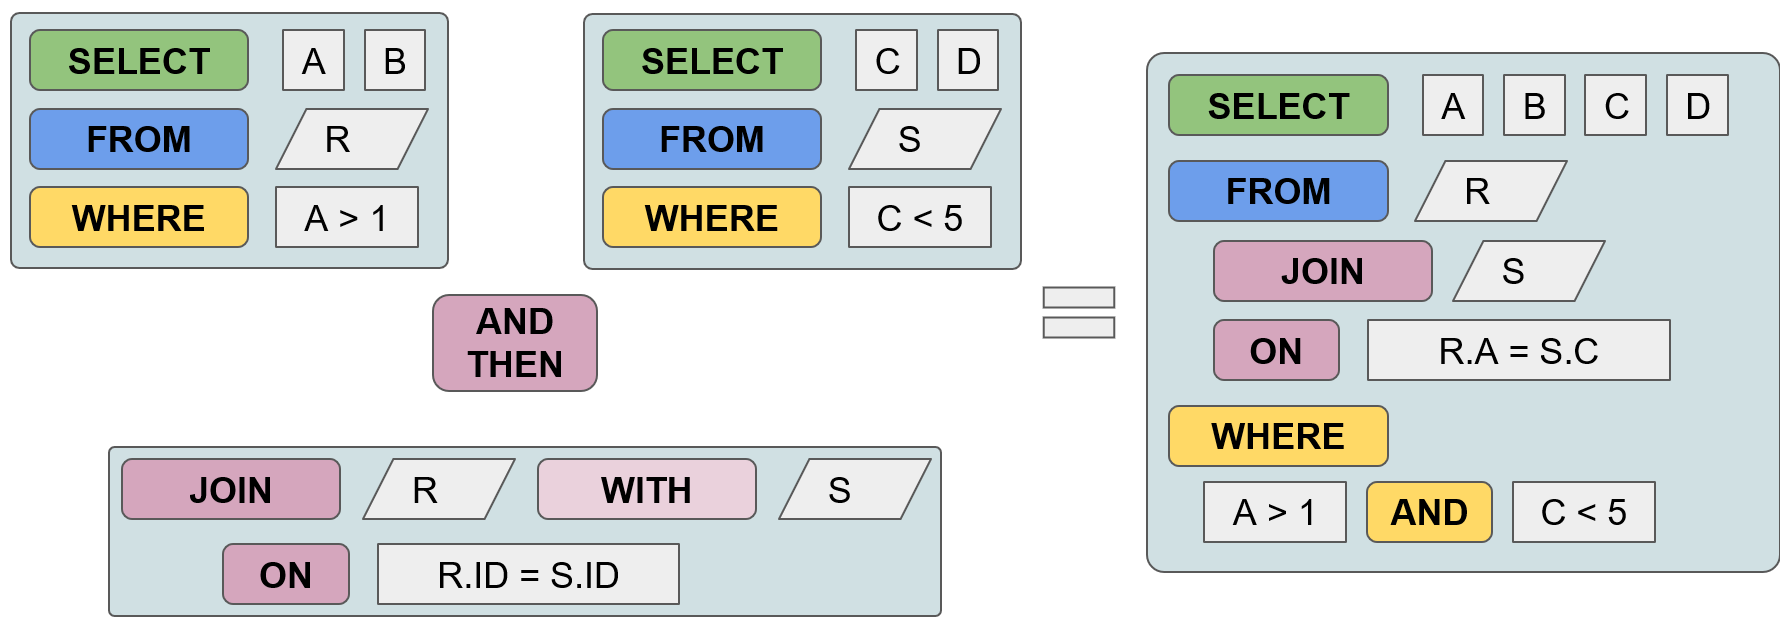
\includegraphics[width=0.6\linewidth]{figures/unbundling_1.png}
  \caption{Query Unbundling}
  \label{fig:unbundling}
\end{figure}

This features aims to make it easier to formulate more complex queries joining multiple tables. 
In SQL, the SELECT clause requires the user to specify \textit{all} columns, scalars, and functions from across all tables in one go, followed by naming \textit{all} table sources, subqueries, and joins in one go, followed by expressing \textit{all} constraints in the form of WHERE predicates. 
Only after all that can the user add modifiers such as LIMIT, ORDER BY, HAVING, and GROUP BY. 
Basically, it is a ``global'' approach to using the full database's schema in query construction.
It forces the retention of a lot of schema details in the speaker's working memory for the entire duration of the query dictation, e.g., all non-aggregate columns that appeared in the SELECT clause must reappear in the GROUP BY clause at the end.
While this may not be a big deal for typing, it can be a hindrance for ease of spoken querying.

Query unbundling aims to directly reduce this cognitive load based on the ``stream of thought'' philosophy inspired by functional programming APIs such as Python Pandas and Spark DataFrames.
Basically, this is a ``local-first'' approach to using the database schema in query construction. 
It is closer to the logical query plan produced behind the scenes for SQL queries. 
We extend the grammar to permit the expression of \emph{unbundled SELECT} queries that specify columns, table source, and WHERE predicates for \textit{one relation at a time}. 
These unbundled relation can then be joined together using separate \emph{join-with} clauses where the speaker defines the join predicate(s). 
Each unbundled query is delimited by the AND THEN, THEN, or NEXT keywords.
Modifier clauses can be specified together in a single expression or separately using multiple modifier clauses. 
The order of the \emph{unbundled SELECT}, \emph{JOIN-WITH}, and \emph{modifier} clauses remains optional, retaining the additional flexibility for dictation that SpeakQL offers.

\paragraph{Query Prompt} Find the titles of all courses offered in terms with the year 2022. 

\paragraph{SpeakQL} 
\emph{
  \textbf{join the} term \textbf{table with the} room \textbf{table on} term dot id equals courseoffering dot termid \\
  \textbf{and then}
  \textbf{join the} courseoffering \textbf{table with the} course \textbf{table on} courseoffering dot courseid equals course dot id \\
  \textbf{and then}
  \textbf{show me} title \textbf{in the} course \textbf{table} \\
  \textbf{and then}
  \textbf{from} room \textbf{where} floor equals 3 \textbf{select average} capacity \\
  \textbf{and then}
  \textbf{get} nothing \textbf{from} term \textbf{where} year equals 2022
}
\begin{verbatim}
  SQL: Select title from course
       join courseoffering 
          on course.id = courseoffering.courseid
       join term 
          on courseoffering.termid = term.id
       where year = 2022;
\end{verbatim}

\subsubsection{\textbf{Unbundled Query Parts}}

There are 3 types of unbundled query parts: a single-relation select-project, a join clause that specifies the join criteria between two single-relation queries, and a modifier clause that enables specification of GROUP BY, HAVING, LIMIT, and ORDER BY.

Within a single-relation select-project clause, a relation can be defined as a table reference or a subquery. 
Projections are expressed within the SELECT clause; and selections relating to the query's relation are defined within the WHERE clause as usual. 
As with non-unbundled SpeakQL queries, the table expression, SELECT expression, and WHERE expression may be dictated in any order. 
Table items for unbundled query parts that contain joins are consolidated in the output SQL query as a combination of a FROM clause for a single table and join expressions for the remaining tables. 
Otherwise, table items for unbundled queries where join conditions between tables are defined within a single-table part's WHERE clause are consolidated in the output SQL query's WHERE clause in the same fashion.
We present two examples.


%Example query
\paragraph{Unbundled SpeakQL query:} \emph{SELECT a and b FROM table R AND THEN GET c and d FROM S WHERE R.id = S.id}
\begin{verbatim}
  SQL: SELECT R.a, R.b, S.c, S.d FROM S, R WHERE R.id=S.id;
\end{verbatim}

\vspace{2mm}
%Example query
\paragraph{Unbundled SpeakQL query:} \emph{SELECT a and b FROM table R AND THEN GET c and d FROM S AND THEN JOIN R WITH S on R.id=S.id}
\begin{verbatim}
  SQL: SELECT R.a, R.b, S.c, S.d FROM S JOIN R on R.id=S.id;
\end{verbatim}

\vspace{2mm}
All 4 queries above are logically equivalent, representable using the relational algebra expression shown below.
The first line lists the individual unbundled queries in SpeakQL that perform the individual projections on $R$ and $S$ first before adding the equi-join part. (NB: We overload $\pi$ for non-deduplicating project in bag semantics for brevity sake.)

%\simpleunbundlealgebra
    \begin{flalign}
        \nonumber [\pi_{a, b}(R)]
        \&\& [\pi_{c, d}(S)]
        \&\& [R \bowtie_{P.id=S.id} S] \\
        \mapsto \pi_{R.a, R.b, S.c, S.d}(R \bowtie_{R.id=S.id} S)
        \label{alg:simpleunbundle}
    \end{flalign}


The above expression introduces two non-standard symbols to represent unbundled queries: square brackets $[$ and $]$ encase individual unbundled query parts, while the double ampersand $\&\&$ is the delimiter of the unbundled query parts, representing the AND THEN keyword or equivalent synonyms in SpeakQL. 
No other operations, say, relational algebra operations, are permitted in between the individual unbundled parts.


\subsubsection{\textbf{Translating an Unbundled Query to SQL}}


Our SpeakQL-to-SQL translator consolidates the unbundled query parts to produce a holistic valid SQL query.

First, column projections, function calls, and function arguments from all single-relation select-project unbundled parts are consolidated together into a single SELECT clause for the output SQL query.
To avoid ambiguity in column names from different tables that are identical strings, every column reference in either a SELECT clause or WHERE clause that is not already in table-prefixed format (i.e., table.column) is prepended with its source table during the translation. 
This is shown in the examples above in which the translated SQL converts reference of column, say, ``a'' in SpeakQL to ``R.a'' in SQL.
If the column reference already prefixes the table, our translator leaves it as is.

Second, selection predicates in the WHERE clauses of individual single-relation select-project query parts are consolidated into a single WHERE clause in the output SQL query using a boolean AND. 
A complex situation arises for a cross-table selection predicate within a boolean expression. 
In such cases, we only support \textit{conjunctive} relationships between single-relation components of the overall boolean expression. 
That is, if a single-relation select-project query part contains multiple selections, these selections are encapsulated in parentheses prior to consolidation within the output SQL query. 
We currently do not support cross-table disjunctive predicates due to the additional complexity they add for speaking and anecdotally such cases being rarer in practice. 
As such, users always have the option of falling back on regular SQL syntax in SpeakSQL for such cases.




\paragraph{\textbf{Detailed Example}}

Figure~\ref{fig:unbundling} illustrates how an unbundled SpeakQL query with two separate single-table WHERE clauses gets consolidated into a single SQL query. The relational algebra representation for both queries is given below.

\eat{
%Example query
\paragraph{Unbundled SpeakQL query:} \emph{SELECT a and b FROM table R AND THEN GET c and d FROM S WHERE R.id = S.id}
\begin{verbatim}
  SQL: SELECT R.a, R.b, S.c, S.d FROM S, R WHERE R.id=S.id;
\end{verbatim}

The SpeakQL query represented in formula \ref{alg:predicateunbundle} on relations $R$ and $S$ \emph{SELECT a and b FROM R WHERE a = 2 OR b = 1 AND THEN GET c FROM S WHERE d < 3 AND THEN JOIN R WITH S ON R.id = S.id} translates to \emph{SELECT R.a, R.b, S.c FROM R JOIN S ON R.id=S.id WHERE (R.a = 2 OR R.b = 1) AND (S.d < 3)}.
}

    \begin{flalign}
        \nonumber [\pi_{a, b}(\sigma_{a > 1}(R))]
        \&\& [\pi_{c, d}(\sigma_{c < 5}(S))]
        \&\& [R \bowtie_{R.id=S.id} S] \\
        \mapsto \pi_{R.a, R.b, S.c, S.d}(\sigma_{((a > 1) \land (c < 5))}(R \bowtie_{R.id=S.id} S))
        \label{alg:predicateunbundle}
    \end{flalign}
%\predicateunbundlealgebra
\eat{
    \begin{flalign}
        \nonumber [\pi_{a, b}(\sigma_{a=2 \lor b=1}(R))]
        \&\& [\pi_{c}(\sigma_{d < 3}(S))]
        \&\& [R \bowtie_{R.id=S.id} S] \\
        \mapsto \pi_{R.a, R.b, S.c}(\sigma_{(a=2 \lor b=1) \land (d < 3)}(R \bowtie_{R.id=S.id} S))
        \label{alg:predicateunbundle}
    \end{flalign}
}

\vspace{2mm}
\subsubsection{\textbf{Selections Without Projections}}

One tricky situation in unbundling arises when a selection predicate (WHERE clause) is applied to a relation from which no columns are returned, i.e., it has no SELECT clause. 
This can lead to an ``odd'' impulse for a query speaker when nothing is retrieved from a table despite it having its own unbundled query part. 
To handle this situation, we introduce the NOTHING keyword as a special token within the \emph{selectExpression} parser rule in the SpeakQL grammar. 


%Example query
\paragraph{SpeakQL:} \emph{FROM TABLE R SHOW ME a AND THEN GET NOTHING FROM S WHERE b = 2 and R.id=S.id}

\vspace{2mm}
\begin{verbatim}
  SQL: SELECT R.a FROM R, S WHERE R.b=2 and R.id=S.id
\end{verbatim}


\vspace{1mm}
\subsubsection{\textbf{Automatic Group By Aggregation}}

To help reduce possible errors from incorrect GROUP BY clauses, we introduce the AUTOMATIC or AUTOMATICALLY keywords. 
The expression GROUP BY AUTOMATICALLY lets the translator infer the output SQL query's GROUP BY clause directly from the SELECT clauses of the unbundled query parts.

%Example query
\paragraph{SpeakQL:} \emph{SELECT a AND THE SUM OF b FROM TABLE R AND THEN GET c and d FROM S AND THEN JOIN R WITH S on R.id=S.id AND THEN GROUP BY AUTOMATICALLY}

\vspace{2mm}
\begin{verbatim}
  SQL: SELECT R.a, SUM(R.b), S.c, S.d FROM R JOIN S
  on R.id=S.id GROUP BY R.a, S.c, S.d
\end{verbatim}


\vspace{1mm}
\subsubsection{\textbf{Verbosity vs.~Brevity}} 

In general, unbundled queries may contain more tokens than their corresponding SQL query, which means they may take slightly more time than reading the pure SQL translation. 
So, the higher naturalness comes at the cost of higher verbosity. 
This is an explicit tradeoff we made based on the rationale that perhaps less ``think time'' may be needed for the ``local-first'' unbundled SpeakQL query than the ``global'' SQL query.
We view this tradeoff as reasonable to both reduce the chance of semantic errors and raise the user's overall query dictation experience.



\paragraph{\textbf{Longer Detailed Example}}

%Example query
The English prompt is as follows: ``What is the average room seating capacity of rooms in buildings where the course with id 'CSE 232' has ever been offered?''.

\paragraph{SpeakQL} 
\emph{
  \textbf{Get} buildingname \textbf{from} building \\
  \textbf{and then}
  \textbf{from the} room \textbf{table where} floor equals 3 \textbf{show me the average} capacity \\
  \textbf{and then}
  \textbf{get} nothing \textbf{from} courseoffering \textbf{where} courseid equals quote CSE232 quote \\
  \textbf{then}
  \textbf{join} courseoffering \textbf{with} room \textbf{on} courseoffering dot roomid equals room dot id \\
  \textbf{next}
  \textbf{join} room \textbf{with} building \textbf{on} room dot buildingid equals building dot id \\
  \textbf{and then}
  \textbf{group by} automatically
}

\begin{verbatim}
  SQL: SELECT buildingname, AVG(capacity)
       FROM courseoffering
       JOIN room ON courseoffering.roomid = room.id
       JOIN building ON room.buildingid = building.id
       WHERE (courseoffering.courseid = 'CSE232')
          AND (room.floor = 3)
       GROUP BY buildingname;
\end{verbatim}




\section{Implementation}


\subsection{Language Specification}

SpeakQL's grammar is defined by extending the modified Backus-Naur Form (BNF) of the MySQL grammar on the ANTLR GitHub repository~\cite{antlrgrammarsv4,Parr2014}. 
We use a subset of rules nested beneath the \emph{querySpecification} parser rule, which are rules within the \emph{dmlStatement} rule set. 
This is similar in size to the SQL subset supported in SpeakQL 1.0~\cite{Shah2020}. 
While the majority of the MySQL grammar in this subset is reused as is, our major changes are within the \emph{selectStatement} and \emph{querySpecification} parser rules and their descendants.

\paragraph{\textbf{Grammar Extension Strategy.}} 
Our general strategy is to add intermediate rules between terminal token nodes and their parent SQL parser rules in order to modularize the grammar in a way that enables the SpeakQL-to-SQL translator to manipulate the abstract syntax trees (ASTs). 
This results in deeper ASTs and may result in a tradeoff between modularity and performance. 
Since SpeakQL is meant for spoken querying, near-realtime performance is an important design factor. 
To combat performance degradation due to deeper ASTs, we pruned the source MySQL grammar to include only DML parse rules. 
Within the DML parse rules, we further pruned out rules that were unlikely to be used during speech dictation.

\paragraph{\textbf{Grammar.}}
We present an excerpt of the grammar for the most complex feature of SpeakQL, query unbundling, in Figure~\ref{fig:unbundlegrammar}.
%The \emph{'?'} symbol appended to a rule indicates that the rule is optional. 
%The \emph{'*'} symbol indicates that zero to many applications of a rule are allowed. 
Symbols or tokens in double quotes mean the content enclosed is a terminal symbol. 
The grammar contains a subset of child and descendant rules relevant to the unbundling feature. 
The root query specification rule, abbreviated as \emph{querySpec}, is the point at which queries that use the unbundling feature diverge.

Unbundled queries may lead with any of the three unbundled query part type rules--\emph{multiJoinExpr}, \emph{selModExpr}, or \emph{unbdQryOrdSpc}--followed by the \emph{exprDelim} rule that contains the \emph{AND THEN}, \emph{THEN}, and \emph{NEXT} terminal tokens. 
Although unbundled and non-unbundled SpeakQL queries may share the parser rules that describe SELECT clauses and WHERE clauses, unbundled queries have distinct FROM clause rules. 
The \emph{tabExprNoJoin} and \emph{fromClsNoJoin}, as their names suggest, omit any possible join expressions. That ensures that individual unbundled query parts reference only one table and leaves the join operations to the \emph{multiJoinExpr} rule and its descendants.
The following Figures \ref{fig:unbundlegrammar} through \ref{fig:selectexprgrammar} contain the grammar for all of the SpeakQL features described in this section.

\begin{figure}[H]
  \unbundleQueryTable
  \caption{SpeakQL Unbundled Query Grammar Excerpt}
  \label{fig:unbundlegrammar}
\end{figure}

\begin{figure}[H]
\synonymgrammartable
\caption{SpeakQL Synonym Keywords Grammar Excerpt}
\label{fig:synonymgrammar}
\end{figure}

\begin{figure}[H]
\whereExpressionTable
\caption{SpeakQL Where Expression Grammar Excerpt}
\label{fig:wheregrammar}
\end{figure}

\begin{figure}[H]
\tableExpressionTable
\caption{SpeakQL Table (From) Expression Grammar Excerpt}
\label{fig:tablegrammar}
\end{figure}

\begin{figure}[H]
\selectModifierTable
\caption{SpeakQL Select Modifier Expression Grammar Excerpt}
\label{fig:modifiergrammar}
\end{figure}

\begin{figure}[H]
\naturalFunctionTable
\caption{SpeakQL Natural Function Expression Grammar Excerpt}
\label{fig:naturalfunctiongrammar}
\end{figure}

\begin{figure}[H]
\sqlSelectStatementTable
\caption{SQL Select Statement Grammar Excerpt}
\label{fig:sqlselectgrammar}
\end{figure}

\begin{figure}[H]
\selectStatementTable
\caption{SpeakQL Select Statement Grammar Excerpt}
\label{fig:speakqlselectgrammar}
\end{figure}

\begin{figure}[H]
\selectExpressionTable
\caption{SpeakQL Select Expression Grammar Excerpt}
\label{fig:selectexprgrammar}
\end{figure}

Figures \ref{fig:speakqlselectgrammar} and \ref{fig:sqlselectgrammar} are excerpts of SpeakQL and SQL select statement grammar in a modified BNF format. The \emph{'?'} symbol appended to a rule indicates that the rule is optional. The \emph{'*'} symbol indicates that 0 to many occurences of a rule are allowed. Symbols or tokens surrounded by double quotes indicate that the content enclosed within the quotes is a terminal symbol. Both figures contain only a subset of child and descendant rules and both are limited to two levels of depth below the \emph{selectStatement} rule, and certain SQL rules including \emph{union}, \emph{window}, and \emph{into} are omitted for the sake of brevity. Figure \ref{fig:selectexprgrammar} is an example of a child expression to the SpeakQL select statement grammar defined in figure \ref{fig:speakqlselectgrammar} and is provided as an example implementation of the extension strategy that facilitates SpeakQL to SQL translation.


\subsection{SpeakQL to SQL Translation}

\begin{figure}[h]
  \centering
  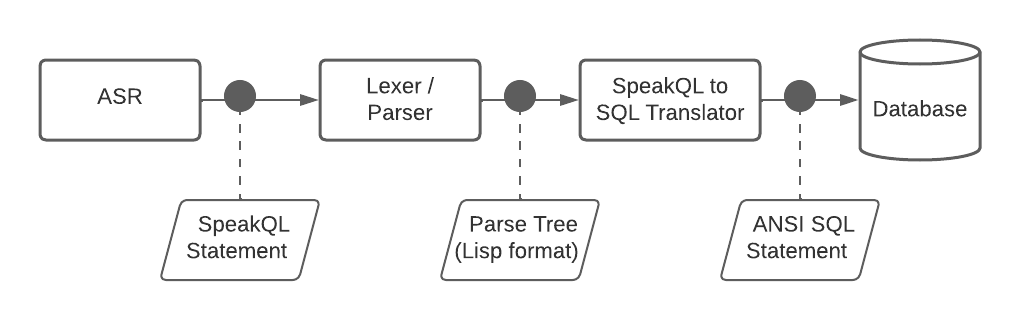
\includegraphics[width=0.8\linewidth]{figures/SpeakQL 2 to SQL Translation}
  \caption{ASR to SpeakQL to SQL translation workflow.}
  \label{fig:translationprocess}
\end{figure}

Our translator takes a valid SpeakQL query as input and returns a semantically equivalent SQL query. Figure~\ref{fig:translationprocess} shows its place in the overall workflow. 
The translator performs a series of steps that we summarize next. 

The translator performs translation through a series of steps. The first step takes a valid SpeakQL query as input, where correctness is determined upstream of this task, and sends it to the Java-based SpeakQL parser via an HTTP post request. The parser responds with a Lisp-formatted abstract syntax tree AST that the Python-based translator transforms into an editable AST. The translator performs operations on the SpeakQL AST in order to transform it into a valid SQL query which include finding and replacing SpeakQL synonyms with SQL syntax, reordering expressions, reordering modifier items, and transforming unbundled queries into a single SQL select statement. The unbundling transformation step includes additional substeps including inference of a group by expression, consolidation of select elements (i.e. columns, functions, and scalars), consolidation of where statements, consolidation of join expressions, and finally consolidation of any table sources not included within join expressions.



\paragraph{\textbf{Synonym Replacement}} 
In this step performs a scan search of all active nodes in the AST for rules that are a member of the keyword and delimiter categories for which SpeakQL synonyms exist. 
This includes \emph{selectKeyword}, \emph{fromKeyword}, \emph{selectElementDelimiter}, and more. 
When a keyword or delimiter rule is identified during the search, the translator performs an update on the rule node that replaces the terminal token representative of a SpeakQL synonym with its corresponding SQL keyword. 
Optional keywords such as THE and TABLE are identified in the same manner and removed from the AST.

\ReplaceSynonymsAlgorithm

\paragraph{\textbf{Clause Reordering}}
This step includes reordering SELECT, FROM, WHERE, GROUP BY, ORDER BY, HAVING, and LIMIT clauses. 
The translator takes advantage of AST structures that guarantee that all children of the \emph{queryOrderSpecification}, \emph{unbundledQueryOrderSpecification}, and \emph{selectModifierExpression} parser rule nodes are rules that require evaluation and reordering. 
Specifically, it is guaranteed that the query order clause parser rules will only contain the children \emph{selectExpression}, \emph{whereExpression}, and \emph{tableExpression}. 
We also know that the \emph{selectModifierExpression} has no more than four children of type \emph{selectModifierItem}, each of which may have a single child of type \emph{groupByClause}, \emph{havingClause}, \emph{orderByClause}, or \emph{limitClause}. 
With these guarantees, the translator simply collects and reorders the AST's parser rules' children into the correct SQL clause order.

\ReorderParseTreeAlgorithm
\ReorderModifiersAlgorithm

\paragraph{\textbf{Natural Function Transformation}}
Translating natural functions to valid SQL function clauses involves locating and removing the optional keyword parser rules and inserting parentheses for all occurrences of the \emph{noParenAggregateWindowedFunction} parse rule in the AST.

\TransformNaturalFunctions

\paragraph{\textbf{Query Bundling}}
This is a series of up to 5 steps to consolidate a set of unbundled query parts into a valid SQL query. 
The number of steps varies by query and is dependent on the presence of WHERE clauses, JOIN clauses, and aggregate function calls. 
The steps in order are:

\begin{enumerate}
\item Infer GROUP BY clause, if any.

\item Bundle SELECT clauses. 

\item Bundle WHERE clauses, if any.

\item Bundle JOIN clauses, if any.

\item Bundle all tables, if more than one.

\end{enumerate}


\paragraph{Translating Unbundled Queries}

The translator uses the same approach for each bundling step, which is to identify the first expression parser rule node in the AST for a given expression and use it as a migration target for additional expression parser rule nodes that may exist in the AST. For example, if a query contains two separate unbundled select-from-where queries connected with a join query, the translator will designate the first of the two \emph{selectExpression} parser rules in the AST as \emph{selectExpression'} and will migrate the \emph{selectElements} that are children of the second \emph{selectExpression} rule node to become children of \emph{selectExpression'}. 
Parser rule node migration is accomplished by appending the migrated parser rule node's ID to the migration target rule node's child list and removing the migrated parser rule node's ID from the migration source rule node's child list.

\TransformUnbundledQuery


% -------------- Tech Report Algorithms and Explanations: -------------------
\paragraph{Inferring the group by expression}

A feature of the SpeakQL translator is its ability to infer a group by expression using the presence of aggregator functions and column references within multiple \emph{selectExpression} parser rules. A user can instruct the translator to perform group by expression inference using the \emph{group by automatically} keyword within either a single-table SpeakQL query or a multi-table unbundled query.

\TransformFunctionInferGroupBy

When the translator encounters the \emph{group by automatically} instruction, it proceeds as depicted in algorithm \ref{alg:infergroupby}. It makes use of AST helper functions \emph{nodeWithName} which returns a list of all nodes with a given rule name, and \emph{getAllTablesAndElements} which returns a Python dictionary (\{ \emph{table name} : [ \emph{selectElements} ]\}) that contains a list of select elements and function calls for each table referenced within the SpeakQL query. The translator uses the existing \emph{groupByExpression} parser rule node that contains the \emph{auomaticGroupByKeyword} parser rule and replaces the \emph{automaticGroupbyKeyword} rule with a \emph{groupByItems} parse rule. The \emph{groupByItems} parse rule node serves as the parent node for individual \emph{groupByItem} and \emph{groupByItemDelimiter} nodes generated from non-function \emph{selectElement} nodes registered in the table-element python dictionary. Because the \emph{groupByItems} parse rule already exists beneath the \emph{selectModifierExpression} parse rule, no further AST transformations are required; and the group by inference operation is complete after the generation of the \emph{groupByItems} parse rule and its children \emph{groupByItem} and \emph{groupByItemDelimiter} parse rules.

\paragraph{Bundling select elements}

Select element bundling is a required step for any SpeakQL query that makes use of the unbundling feature. Because any SpeakQL query that uses unbundling must have at least two \emph{selectExpression} parse rules, select element bundling is a mandatory step of the bundling process.

\TransformFunctionSelectElements

As shown in algorithm \ref{alg:transformfunctionselectelements} as \emph{selElmtsRlNd'}, which abbreviates \emph{selectElementsRuleNode}, the translator uses the first \emph{selectElements} parser rule as a migration target for all other select elements within the SpeakQL query. Also depicted in the same algorithm is a preemptive method for avoiding ambiguity where the translator prepends each migrated select element with its associated table, resulting in a dotted id in the format \emph{tableName.columnName}. This step is performed for both standalone column references and column references as arguments within function expressions. After iterating through each \emph{selectElementExpression} parser rule and migrating their associated \emph{selectElements} children to \emph{selectElementsRuleNode'}, a cleanup operation removes them from the AST leaving a single \emph{selectElementsExpression} in the AST that contains all column and function references present in the original SpeakQL unbundled query.

\paragraph{Bundling where expressions}

The where expression bundling step is optional, and is only invoked if at least one bundled query expression contains a \emph{whereExpression} parse rule. When performing where expression bundling, the SpeakQL translator makes the following assumptions:

\begin{itemize}
\item All cross-table predicates are conjunctive (and)
\item Multiple predicate expressions within a single unbundled query should be encased in parentheses before consolidation
\end{itemize}

Given these assumptions, where expression bundling proceeds as depicted in algorithm \ref{alg:transformfunctionwherestatements}.

\TransformFunctionWhereStatements

Similar to the select element bundling step, the first occurence of a \emph{whereExpression} parse rule, \emph{whereExpression'}, within the query AST and designates it as the target for additional \emph{whereExpression} parse rule migration. Because where expressions are optional within \emph{selectStatement} parser rules, it is possible that \emph{whereExpression'} is not a member of the first \emph{selectStatement} parse rule, \emph{selectStatement'}, in the query. Because of this possibility, the translator may perform an additional migration step where it migrates \emph{whereExpression'} to become a child of \emph{selectStatement'}.

The translator takes advantage of the recursive nature of the where expression grammar (see figure \ref{fig:whereexprgrammar}) by designating where expressions that exist in \emph{selectStatement} parse rules that are not \emph{selectStatement'} as children of \emph{whereExpression'}. During this migration process, the translator employs helper functions to surround migrated expressions with parentheses and deliminating the migrated expressions with \emph{andKeyword} parser rules. The end result of this process is a single cross-table conjunctive \emph{whereExpression} parser rule that contains all other \emph{whereExpression} parser rules specified in other unbundled queries within the SpeakQL query. 

\paragraph{Bundling join parts}

Join part bundling collects all \emph{multiJoinExpression} parse rules and aggregates them in an arbitrary order to form a valid SQL join expression. Join part bundling is an optional feature because an alternate form of relation joining where all table sources are specified within \emph{fromExpression} parse rules, and join conditions between each table source are specified within \emph{whereExpression} predicates (e.g. \emph{from table one, table two where one.id = two.id}), is also possible. Currently, because join order in the resulting SQL query is arbitrary within the bounds of its implementation rules, join part bundling is limited to allowing only inner joins. Queries that require outer join expressions may still be expressed using other SpeakQL features; but may not employ the unbundling feature. Outer join capability is a future SpeakQL feature development objective.

% \TransformFunctionJoinParts

The join part bundling process begins when the translator creates a list of all \emph{multiJoinExpession} parse rule nodes within the AST. Given this list, it performs iterative analysis on each expression to determine if a subquery exists as a table item within any of the \emph{multiJoinExpression} nodes, and if so, substitutes the subquery with a subquery masking rule and alias in the join expression. The translator then checks the left and right table reference parse rules within the join expression to determine if an alias exists for each table, or if the table is referenced in the join expression by its alias. If an alias association is encountered, it creates \emph{asKeyword} and \emph{multiJoinTableAlias} parse rules and adds them as children to the target \emph{joinExpression} parser rule that represents the objective SQL-correct join expression.

After analyzing all \emph{multiJoinExpression} and making modifications toward SQL-correct syntax, the translator begins the join consolidation process by designating the first table referenced in the queries first \emph{selectStatement'} as the base table upon which the SQL-correct join statement will be built. In order to ensure valid join expression chaining, the translator determines a table join order that ensures that each subsequent table added to a join expression references a table in its join condition that already exists within the objective join expression. In other words, while building the SQL-correct join expression, a \emph{multiJoinExpression} will not be added to the target \emph{joinExpression} until all tables referenced in its join condition have been added to the target \emph{joinExpression}. The process will continue iterating over remaining \emph{multiJoinExpressions} until the table existence constraint can be satisfied and all expressions have been added to the objective SQL-correct expression, or it is determined that \emph{multiJoinExpressions} exist in the SpeakQL query that cannot be chained and the translator responds with an error condition. The translator then performs an additional safety check to ensure that all tables referenced in the query's \emph{unbundledQueryOrderSpecification} parser rules are also referenced in a corresponding \emph{multiJoinExpression} parser rule, and throws an error if a violation is encountered.

After the join bundling process is completed, all join expressions consolidated within a single \emph{multiJoinExpression} are migrated to the first \emph{tableExpressionNoJoin} parse rule. The \emph{tableExpressionNoJoin} parse rule name is then updated to \emph{tableExpression} and becomes a valid SQL from + join expression; and join bundling is complete.

\paragraph{Bundling table expressions}

The final step of the bundling process involves collection of all \emph{tableExpressionNoJoin} parse rule nodes within the AST. This is only required in cases where an unbundled query contains multiple table references but has no associated \emph{multiJoinExpression} parser rules. In this case the first \emph{tableExpressionNoJoin}, designated as \emph{tableExpressionNoJoin'}, is established as the expression migration target, and additional \emph{tableExpressionNoJoin} rules that exist as children of additional \emph{selectStatement} rules are added to \emph{tableExpressionNoJoin'}. If a where expression exists in any \emph(selectStatement) that defines a join condition between two tables within the query, the expression consolidation occurs during the previously described where expression bundling step. If no where condition is defined between two tables within the query, the translator still performs table expression bundling, and the result is a SQL statement that produces a cartesian product of the two tables.

% \TransformFunctionTables

\paragraph{Syntax tree cleanup}

After all relevant bundling steps are complete, the translator performs syntax tree cleanup by removing parse rules from which their child sub expressions have been migrated. Upon completion of tree cleanup, the SpeakQL to SQL translation process is complete, and serialization of the abstract syntax tree's terminal nodes results in a valid SQL statement equivalent to the input SpeakQL query.


\paragraph{\textbf{SpeakQL Parser Performance Comparisons}}
A comparison of the SQL and SpeakQL grammar implementations reveals that SpeakQL feature implementation results in deeper trees with additional branches. Naturally, this increase in complexity will result in a corresponding increase in time required to parse a query. A performance comparison between three parsers, a MySQL grammar-based parser, a full SpeakQL parser that extends the entire MySQL grammar, and a simple SpeakQL parser that extends only a DML subset of the MySQL grammar was conducted to validate assumptions about parser performance improvements for smaller grammars. 

\begin{figure}
    \centering
    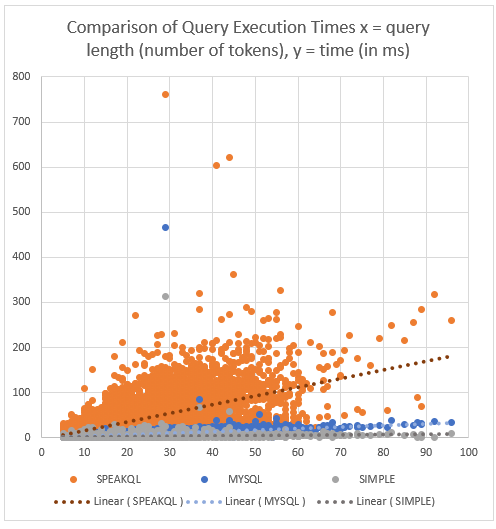
\includegraphics[width=0.5\linewidth]{figures/parser-performance-plot.png}
    \caption{Grammar Parser Performance Comparison}
    \label{fig:parserperformanceplot}
\end{figure}

We measured parse time for each parser using a set of 8,946 SQL queries. The full SpeakQL parser, on average, exhibited a 5.9x \emph{slowdown} compared to the MySQL parser, suggesting that the modularity-based rule extensions negatively impact parser performance. On the other hand, the simple SpeakQL parser extending only a DML subset of MySQL rules exhibited a 2.6x \emph{speedup} compared to the MySQL parser and a 15.1x \emph{speedup} compared to the full SpeakQL parser. This performance increase is achieved by sacrificing certain SQL features including \emph{window} and \emph{union}. This rule omission is mitigated using a fallback strategy where SpeakQL queries identified by the translator as containing syntax not covered by the Simple SpeakQL parser are passed back to the full SpeakQL parser for processing.



\section{User Study}


To evaluate the utility of the SpeakQL dialect, we perform an apples-to-apples comparative A/B user study of \textit{dictating SpeakQL vs.~dictating regular SQL}. 
Our goal is to understand the role of our \emph{dialect's features} on how efficiently one can dictate a syntactically valid query. 
So, we use a ``Wizard of Oz'' strategy to simulate a speech-based interface to allow us to focus only on the dialect's role. 
We do \textit{not} want to confound this evaluation with orthogonal factors such as interface specifics, auxiliary additional modalities such as touch, etc. 
Thus, our goal here is different from the user study conducted for the SpeakQL 1.0 system~\cite{Shah2020}, 
which compared typing SQL on a tablet against speech+touch modality on their multimodal tablet interface. 
We leave it to future work to study how to integrate the SpeakQL dialect into such multimodal interfaces. 


\subsection{Study Objectives}

\subsubsection{\textbf{Research Questions and Hypotheses}}

The user study is motivated by three main research questions. We also posit our hypothesis alongside each question.

\vspace{2mm}
\textit{Q1: Effectiveness of alternate syntax.} To what extent, if any, do syntax synonyms and symbol reduction improve user experience during spoken querying?

\vspace{2mm} 
\textit{H1: Synonyms and reduction in special characters improve user experience.} 
We expect that syntax synonyms and avoiding the need to dictate special characters such as comma, parentheses, or asterisk can make the process feel more natural and reduce number of errors and time taken to dictate simple queries. 

\vspace{2mm}
\textit{Q2: Effectiveness of alternate ordering.} To what extent, if any, does relaxing structure through alternate clause ordering reduce chances of errors during spoken querying?

\vspace{2mm} 
\textit{H2: Alternate ordering reduces errors.} 
We expect that relaxing the ordering requirement among clauses can reduce number of ordering-related syntax errors and reduce the amount of time and number of attempts required to dictate a simple or complex query. 

\vspace{2mm}
\textit{Q3: Effectiveness of unbundling.} To what extent, if any, does unbundling a complex query into smaller single-relation parts reduce chances of errors during spoken querying?

\vspace{2mm} 
\textit{H3: Unbundling reduces burden on working memory.} 
We expect that unbundling a complex multi-table query into single-table query parts can reduce the speaker's working memory burden, reduce chances of errors when speaking the whole query, and reduce the number of attempts to craft a fully correct query.


\subsection{Study Protocol and Design}


\paragraph{\textbf{Participants}}
We recruited participants from academic programs that teach SQL and data analytics.  
Since the SpeakQL dialect is primarily aimed at data professionals who already know SQL (not lay users), we also required participants to be familiar with SQL. They had to complete a short SQL screening test. 
Those who passed the test were invited to join the user study and offered up to \$30 as compensation. 
It was structured as a flat rate of \$6 for joining and \$2 per query prompt completed (both SQL and SpeakQL conditions) for up to 12 query prompts. 
We also attempted to recruit participants from online database- and SQL-focused communities; but no prospective candidates passed the SQL screening questionnaire. This resulted in a set of participants sourced from a single university which, though the university celebrates a very diverse student body, may limit the scope of the study to Anglo-centric and English-only contexts.

\paragraph{\textbf{Managing the Learning Effect}}
We applied a latin squares approach using counterbalancing to attempt to counteract the learning effect that is known to be inherent in within-subjects studies of two or more treatments~\cite{10.5555/2501707}. 
Specifically, participants are divided into two groups: a SpeakQL-to-SQL group and a SQL-to-SpeakQL group. 
All participants in one group answered all 12 questions in one dialect first and then switch to the other dialect.

\paragraph{\textbf{Database Schema and Queries}}
We use a 6-table university course database schema for our user study. 
It is a snowflake schema with a course offerings table at its center with three foreign keys referencing tables on courses, rooms, and terms. 
The course and room tables have foreign keys referencing tables on departments and buildings, respectively.
For practice we created 3 realistic queries of increasing complexity: a single-table project, a single-table aggregate, and a 3-table join. 
The study itself uses 6 simple and 6 complex queries, with all the simple queries being single-table queries, while the complex ones join between 2 and 5 tables each.

\paragraph{\textbf{Logistics}} 
Study sessions were conducted over Zoom with a simple browser-based web interface. 
The interface enables the speaker to see the database schema, receive query prompts, dictate queries through their device's microphone, and see the live ASR transcription of their dictation. 
We use the state-of-the-art Whisper model for ASR~\cite{https://doi.org/10.48550/arxiv.2212.04356}. 
The study administrator employed a separate ``Wizard of Oz'' control panel to evaluate correctness of the spoken query, to offer feedback in realtime (i.e., identify errors and ask for re-dictation if needed), to answer general questions on SQL or SpeakQL, and to manage the overall progression of the study session. 

\paragraph{\textbf{Quantitative Analyses}}
We evaluate performance using the following dependent variables: planning time (time from seeing query prompt to starting recording which accounts for schema review, note taking, questions, and verbal rehearsals), number of attempts till a fully correct query, completion time per attempt, and total completion time for all attempts.
Independent variables are based on query prompt attribute and feature usage. 
Prompt attribute is the complexity of the correct SQL query, binarized as simple or complex (more details below). 
Feature usage determination is based on post-participation transcription of recordings and further analyses. 

\paragraph{\textbf{Measuring Query Complexity}} 
We use a series of weighted criteria: number of relations, number of projection terms (columns, functions and constants in SELECT clause), number of functions, number of predicates (in WHERE clause), number of joins, and number of modifiers (GROUP BY, HAVING, ORDER BY, and LIMIT). 
We use these to derive both raw and standardized query complexity scores. 

\paragraph{\textbf{Determining Feature Usage}} 
For each query attempt, we analyze feature usage post-hoc based on both the ASR transcription and the raw audio recordings. 
We used syntax-focused heuristics on the ASR output text to make this process easier for us, e.g., to check if unbundling was used, we performed a search for at least one ``AND THEN'' in the transcript and coded the attempt based on the presence or absence of that keyword.



\paragraph{\textbf{Study Session Overview}}
Each session was for 90 minutes, and began with a 22 minute training video that provided an overview of SpeakQL features and usage examples. 
Following the video was a brief question and answer session and user interface demonstration.
Participants then answered up to 15 prompts using both dialects (3 practice and 12 measured). 
They dictated in one dialect (SpeakQL or SQL) and then repeated the same queries in the same order for the other dialect. They were encouraged to use as many SpeakQL features as possible. 
The study administrator was available to answer questions about the schema or language syntax.
The online context made a note taking prohibition unenforceable. 
As such, we deemed that a complete restriction would result in a temptation to take notes covertly. 
Participants were advised that they \emph{should} try to perform without using notes, but if they did, they were required to discard them after the first dialect to mitigate learning effect bias.




\section{Results and Discussion}


Our recruiting efforts elicited 35 prospective participants, of which only 30 completed the SQL filtering test.
Of those, 29 were invited to participate and 23 ultimately did. 
Data from one participant was omitted from analysis due to a violation of the note transfer policy. 
19 participants completed all 12 prompts; 3 answered at least 7 prompts in both dialects before opting to end the session.




\subsection{Quantitative Results and Hypotheses Tests}




\paragraph{\textbf{Feature Usage Impact}} 
Hypotheses H1 and H2 are feature-focused tests to analyze the impact of specific SpeakQL features. 
But since SpeakQL feature usage was optional, it turned out that participants did not consistently use many SpeakQL features across many prompts. 
Feature usage was also not consistent between participant groups (SpeakQL-first vs.~SQL-first) and participants who had SQL as their first condition were less likely to use SpeakQL features as often as participants who had SpeakQL as their first condition. 
Due to this unexpected imbalanced voluntary usage rate for some features, we are unable to make any significant observations of feature usage effects on dependent variables. 

\begin{figure*}[t]
  \centering
  \begin{subfigure}{.4\textwidth}
    \centering
    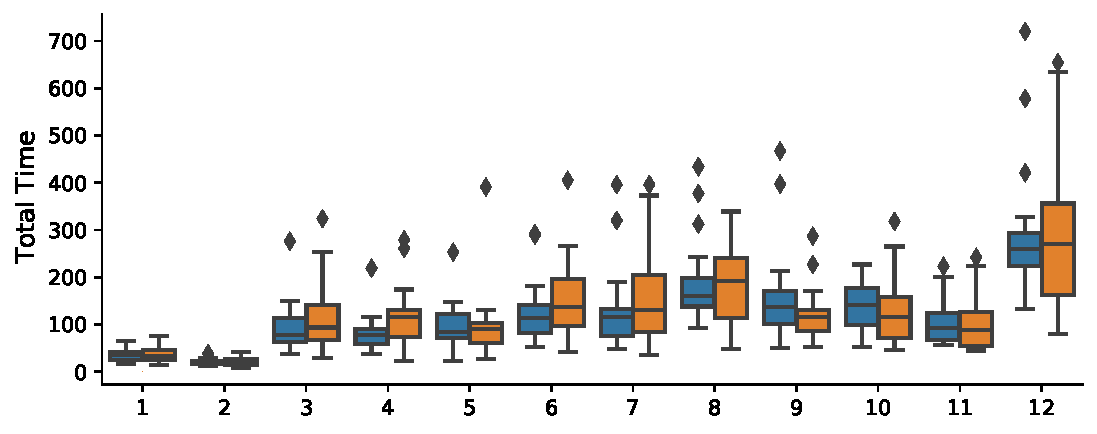
\includegraphics[height=1.0in]{figures/query-total-time-boxplot.pdf}
    \caption{Total Time, All Attempts,\\By Individual Query}
    \label{fig:querytotaltime}
  \end{subfigure}
  \begin{subfigure}{.5\textwidth}
    \centering
    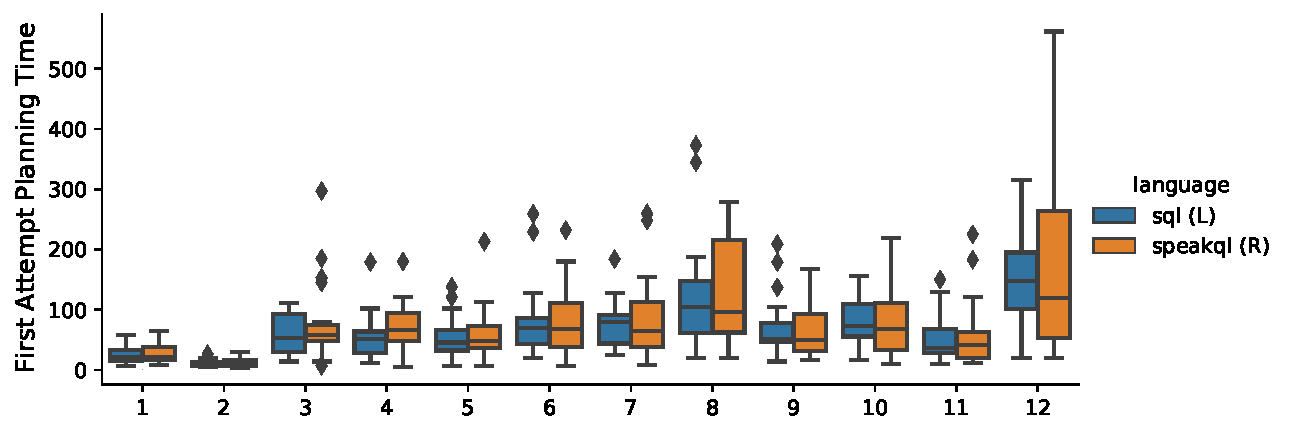
\includegraphics[height=1.0in]{figures/query-planning-time-boxplot.pdf}
    \caption{Planning Time, First Attempts,\\By Individual Query}
    \label{fig:queryplanningtime}
  \end{subfigure}
\end{figure*}

\paragraph{\textbf{Planning Time}} 
Planning time is a part of H1 and H2. 
We analyzed total number of attempts to reach a correct query, as well as the planning time for the first attempt. 
We measure first attempt planning time as opposed to the planning time for the final attempt because our observation was that for second and third attempts, participants generally performed no additional planning.
Thus, the time participants take to digest the prompt, analyze the schema, and plan the query is reflected within the first attempt planning time. 
Figure~\ref{fig:queryplanningtime} shows the distribution for each query. 
The median planning time for simple queries ended up \textit{longer} for SpeakQL than SQL: 38.5s vs.~31.5s, although this difference is not statistically significant (p~=~0.14). (The p-values are derived using the Mann-Whitney U Test.) 
For complex queries, the median planning time is \textit{shorter} for SpeakQL than SQL: 66.0s vs.~72.0s, but again this difference is not statistically significant (p~=~0.295). 
We also compared these results for each individual query and find no statistically significant difference in median planning times for SpeakQL vs.~SQL for any query (p-values between 0.07 and 0.48). 

\begin{figure}[t]
  \centering
  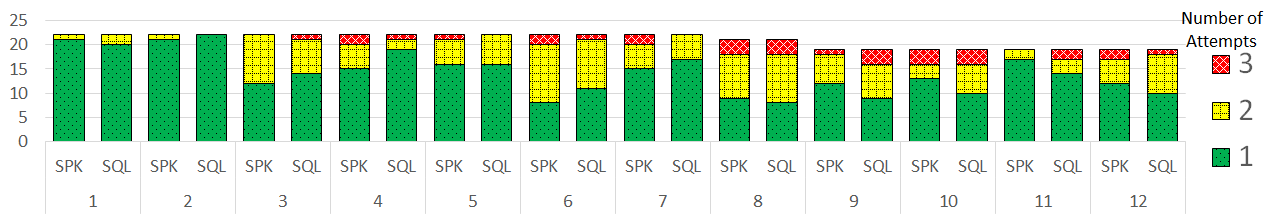
\includegraphics[width=\linewidth]{figures/query-attemptnum-histplot-excel.png}
  \caption{Number of Attempts By Individual Query}
  \label{fig:queryattemptnum}
\end{figure}

\paragraph{\textbf{Number of Attempts}}
This is a part of all three hypotheses. 
Figure~\ref{fig:queryattemptnum} shows the distributions. 
Overall, we do not see any statistically significant differences in either mean or median numbers of attempts between SQL and SpeakQL. 
But we observed that as queries become more complex, more second and third attempts are required. 
However, as the session progressed, first attempt correct answers increased, suggesting that participants gained a familiarity with the query dictation process and that counteracted the increasing query complexity. 
Additionally, we observe a slightly higher improvement advantage for SpeakQL over SQL from queries Q9 to Q12, i.e., the frequency of first attempt correct answers is higher for SpeakQL and that keeps going up.



\subsection{Feature Usage and Usefulness}
\begin{figure}
\begin{subfigure}{\linewidth}
  \centering
  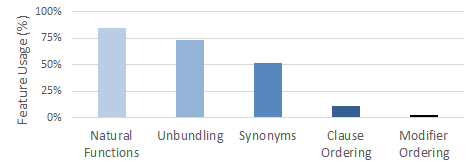
\includegraphics[width=0.8\linewidth]{figures/feature_usage.png}
  \caption{SpeakQL Feature Usage - Observed}
  \label{fig:featureusage}
\end{subfigure}
\begin{subfigure}{\linewidth}
  \centering
  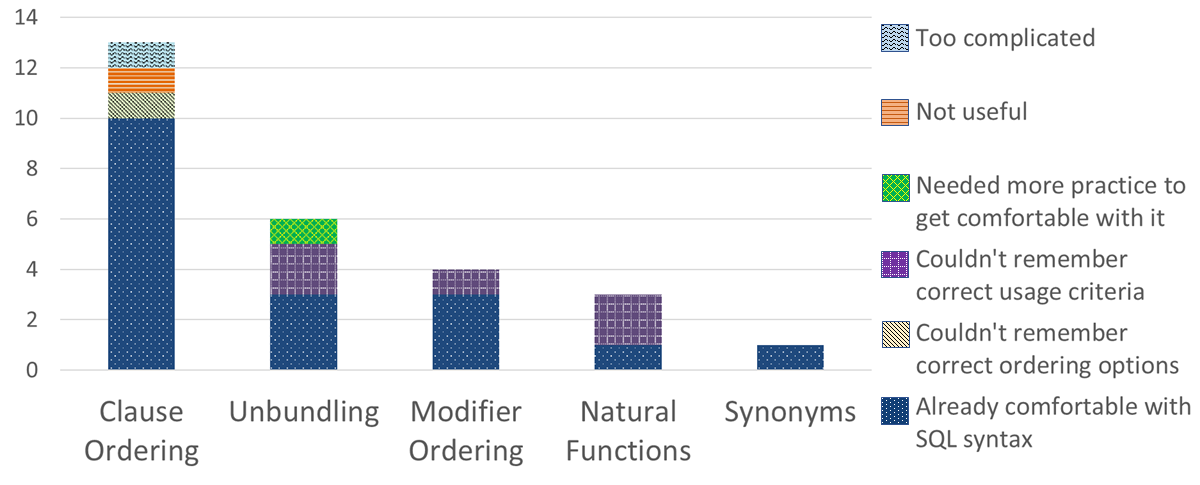
\includegraphics[width=0.8\linewidth]{figures/feature_unused_reasons_excel.png}
  \caption{Participant Reasons for Not Using a Feature}
  \label{fig:unusedfeatures}
\end{subfigure}
\caption{Feature Usage Observations and Avoidance Reasons}
\end{figure}
Analysis of feature usage shows varying levels of popularity for SpeakQL features. 
Since feature usage was optional, some participants relied more heavily on regular SQL syntax than others even for the SpeakQL condition. 
Figure~\ref{fig:featureusage} shows a significant disparity in popularity of the four main features. 
Natural functions are the most popular, followed by unbundling and synonyms; clause and modifier reordering are the least popular. 
Figure~\ref{fig:unusedfeatures} shows the frequency of the self-reported reasons for not using a given feature.
As expected, SQL familiarity is a top reason that dissuaded some participants from using SpeakQL features. 
In particular, clause/modifier reordering were not used due to that reason the most. 
Some also could not remember how to use unbundling or natural functions, perhaps due to their novelty.

\begin{figure}[ht]
  \centering
  \begin{subfigure}{0.5\linewidth}
    \centering
    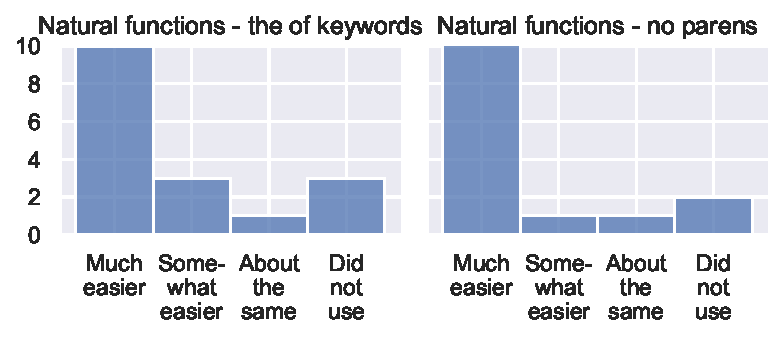
\includegraphics[width=\linewidth]{figures/survey-feedback/function-feedback.pdf}
  \end{subfigure}%
  \begin{subfigure}{0.5\linewidth}
    \centering
    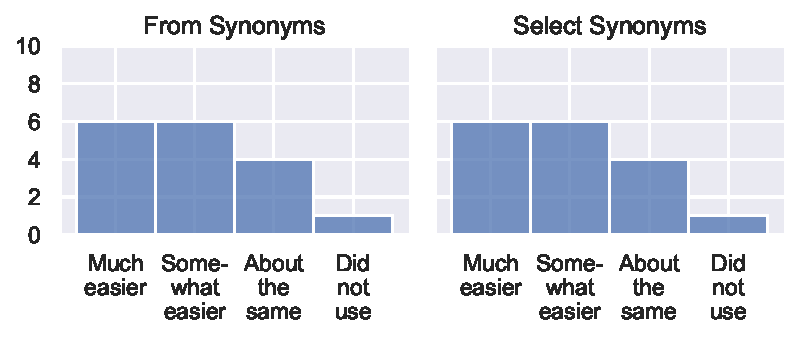
\includegraphics[width=\linewidth]{figures/survey-feedback/synonym-feedback-1.pdf}
  \end{subfigure}
  \begin{subfigure}{0.5\linewidth}
    \centering
    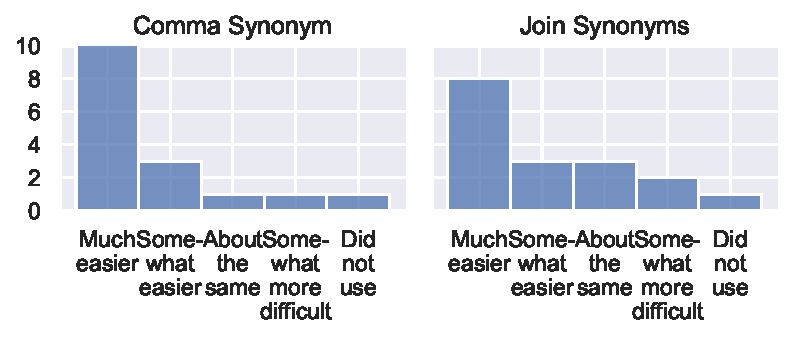
\includegraphics[width=\linewidth]{figures/survey-feedback/synonym-feedback-2.pdf}
  \end{subfigure}%
  \begin{subfigure}{0.5\linewidth}
    \centering
    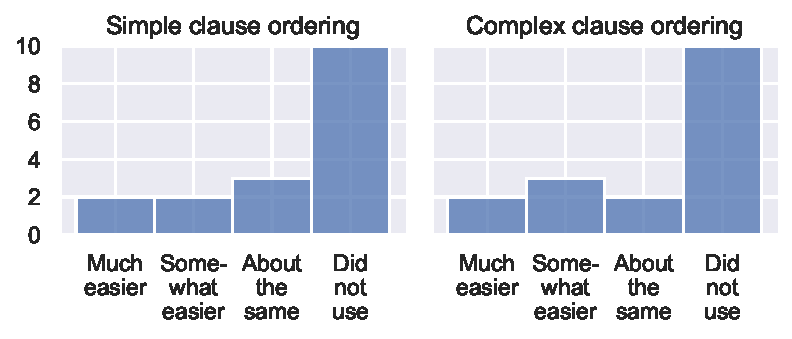
\includegraphics[width=\linewidth]{figures/survey-feedback/ordering-feedback-1.pdf}
  \end{subfigure}
  \begin{subfigure}{0.5\linewidth}
    \centering
    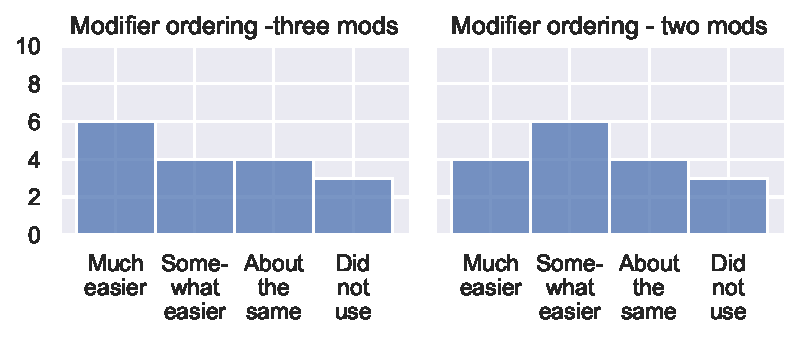
\includegraphics[width=\linewidth]{figures/survey-feedback/ordering-feedback-2.pdf}
  \end{subfigure}%
  \begin{subfigure}{0.5\linewidth}
    \centering
    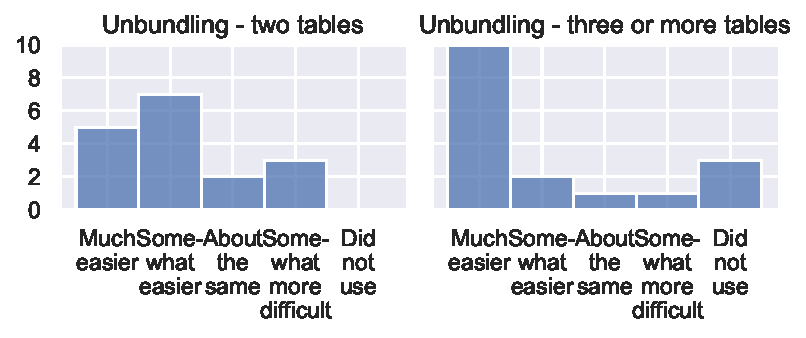
\includegraphics[width=\linewidth]{figures/survey-feedback/unbundling-feedback.pdf}
  \end{subfigure}
  \caption{SpeakQL feature usefulness compared to SQL.}
  \label{fig:surveyusefulnessgraphs}
\end{figure}

We also asked participants who used a feature to rate its usefulness. 
Figure~\ref{fig:surveyusefulnessgraphs} shows the results for all features. 
These results reveal interesting nuances on the low-popularity synonym feature: participants preferred punctuation and join synonyms but they did not care for SELECT or FROM synonyms. 
The other ratings are consistent with the feature usage observations. 




\subsection{Failure Analysis} 

\paragraph{\textbf{Failure Categories}}
We analyzed the transcripts and audio files of incorrect attempts in order to organize failures into the following categories: 1) Syntax, where the participant's query had at least one syntax error (e.g. missing a delimiter or parenthesis, using an invalid keyword, or omitting a clause such as group by); 2) Dictation, where the participant appeared to lose their train of though and terminated their attempt voluntarily; 3) Schema, where the participant referenced a table or column that either did not exist in the schema or was not valid in the context of the clause in which it appeared (e.g. referencing a table instead of a column); 4) Semantic, where the participant's query was syntactically correct but did not return the correct answer.

\begin{figure}
  \centering
  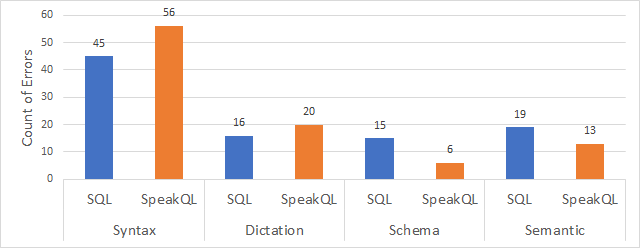
\includegraphics[width=0.8\linewidth]{figures/error-type-counts.png}
  \caption{Attempt error categories by dialect}
  \label{fig:errorcounts}
\end{figure}
\paragraph{\textbf{Observations}}

Figure \ref{fig:errorcounts} shows the breakdown of error types by dialect and failure category. The total number of failures analyzed was 190, 95 SpeakQL and 95 SQL. All failure categories occured for both dialects; but syntax and dictation failures were more commmon for SpeakQL than SQL. Conversely, schema and semantic failures were more common for SQL than SpeakQL. The higher rate of syntax and dictation errors for SpeakQL is likely due to the fact that SpeakQL is a new language and participants were not as familiar with it, though we did observe a much higher rate of SpeakQL syntax errors where participants used incorrect keywords or invalid synonyms. The lower rate of schema and semantic error hints at the possibility that some aspect of SpeakQL may have made it easier for participants to reason about the schema and the query prompt.



\subsection{Learning Effect Impacts on Results}

\begin{figure*}
  \centering
  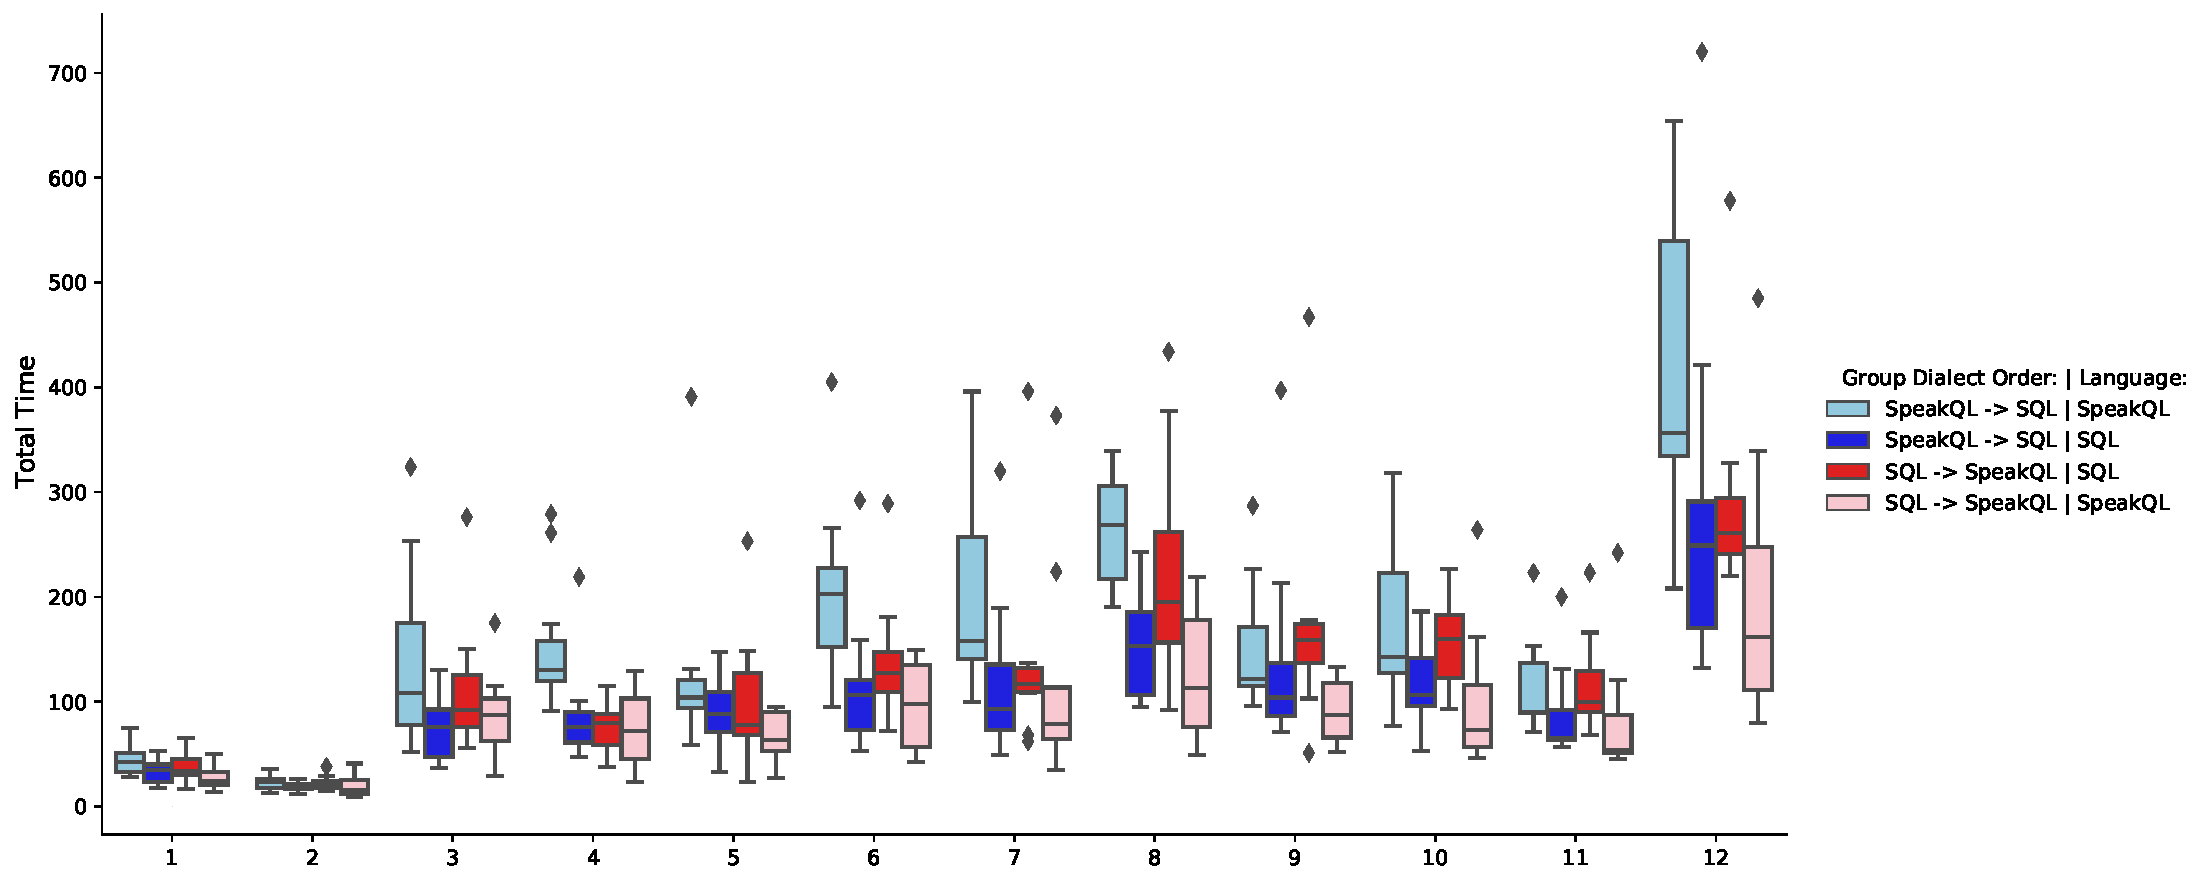
\includegraphics[width=\linewidth]{figures/query-planning-total-time-withgroups-boxplot.pdf}
  \caption{Dialect performance measured by total time and separated by group dialect order.}
  \label{fig:performancebygrouptotaltime}
\end{figure*}

\begin{figure*}
  \centering
  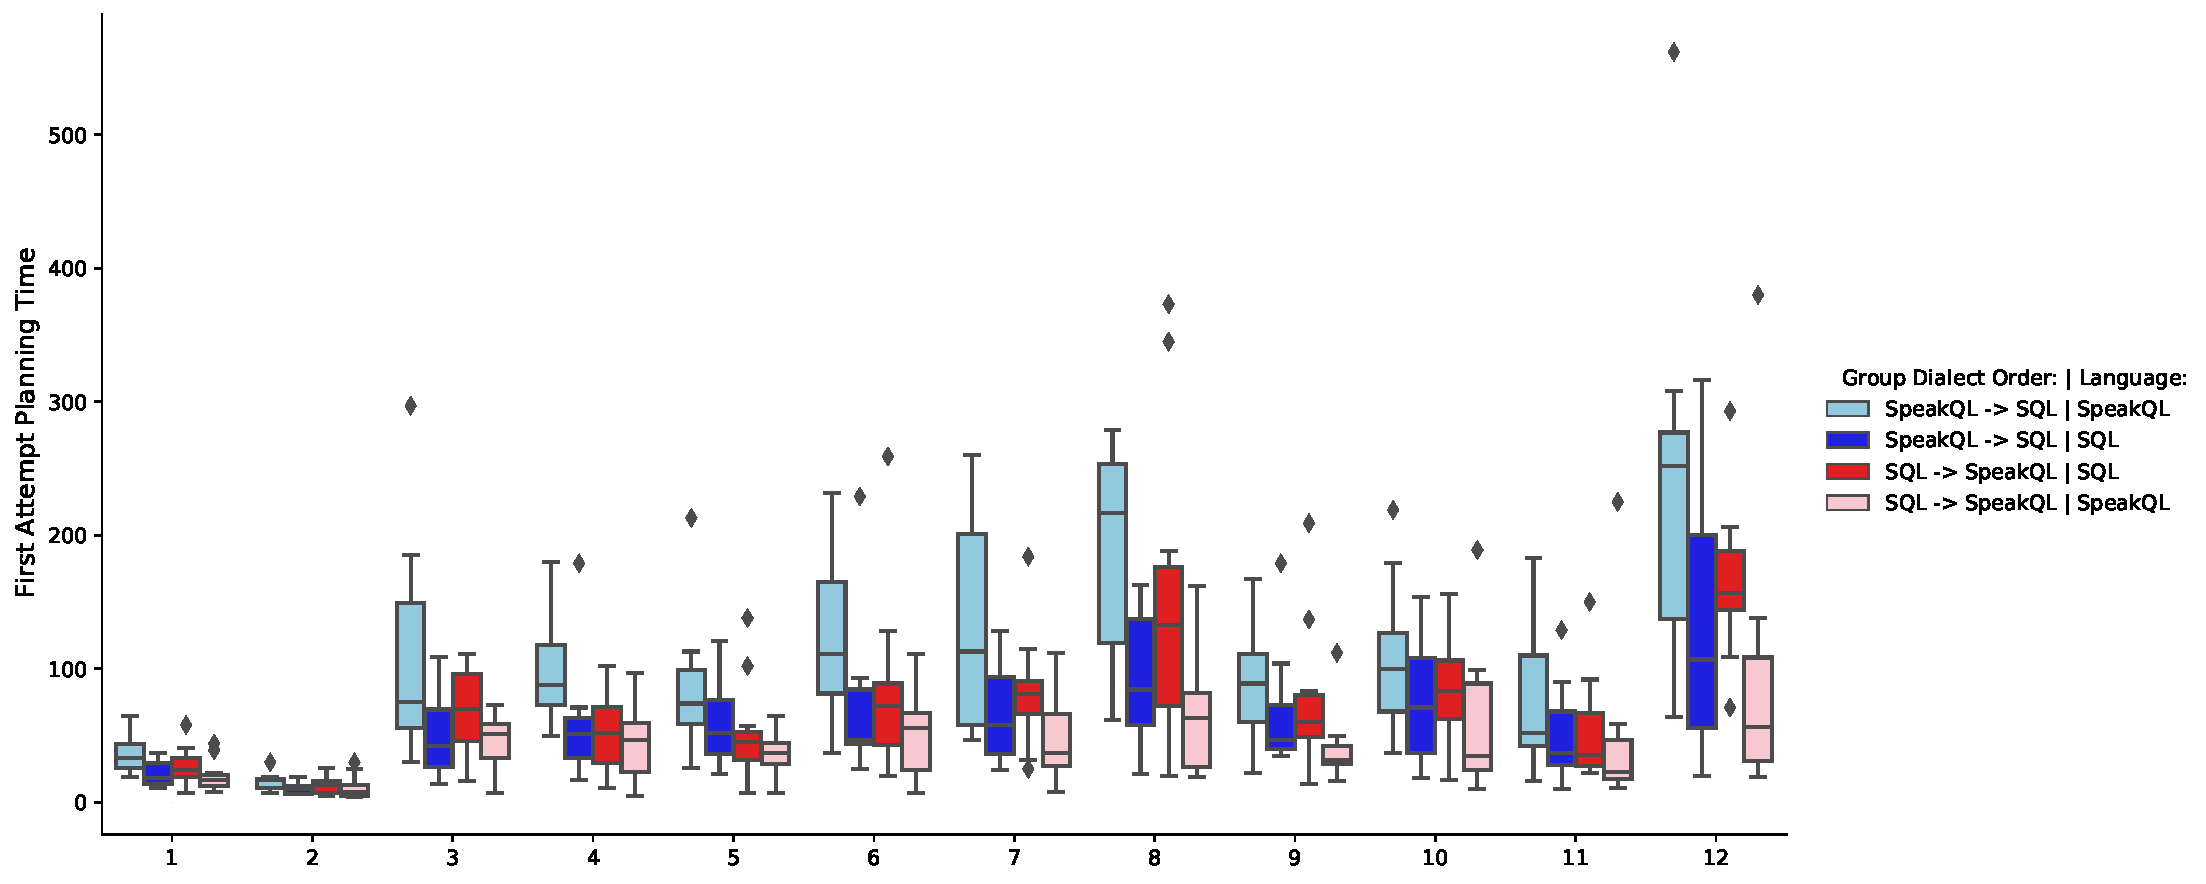
\includegraphics[width=\linewidth]{figures/query-planning-first-attempt-time-withgroups-boxplot.pdf}
  \caption{Dialect performance measured by first attempt planning time and separated by group dialect order.}
  \label{fig:performancebygroupfirstattempttime}
\end{figure*}


During the study design process, we elected to use a within-subjects design in order to reduce the number of participants needed to achieve statistical significance. 
The drawback of this approach is that it introduces a learning effect bias. 
We attempted to mitigate this effect through counterbalancing the dialect order between participants so that half of our participants would have SpeakQL as their first dialect and half would have SQL as their first dialect. 

Despite our learning effect mitigation strategy, we observed evidence of asymmetric learning effects between the two dialects. 
Specifically, members of group 2 (those who used SQL first) exhibited higher improvement using the second dialect relative to their first-dialect performance than members of group 1 (those who used SpeakQL first). 
Figures \ref{fig:performancebygrouptotaltime} and \ref{fig:performancebygroupfirstattempttime} replicate figures \ref{fig:querytotaltime} and \ref{fig:queryplanningtime} but split by participant group and provide an impression of the assymetry between groups. 

Post-hoc analysis of participant data, comparing only first dialect performance between groups, provides an approximate view of the results of what would have been a between-subjects study design, though it is important to note that the study protocol was setup to be within-subjects.
The results of this analysis are not necessarily a valid comparison of the two groups because within-subjects bias reducing design techniques such as participant stratification based on skill levels or other attributes were not implemented. 

With the limitations of the post-hoc between-subjects approximation in mind, we observe that the median first attempt planning time and total attempt time for both simple and complex query types were lower for SQL than for SpeakQL (p value < 0.05 for all observations). 
There were no apparent advantages for either dialect in terms of number of attempts. 
The conclusion we draw from this observation is that should we pursue a more robust between-subjects study design, we would increase the amount of practice and training time for the SpeakQL dialect to help participants become more comfortable with SpeakQL syntax prior to performing measured attempts.
We also consider that the naturalness of the SpeakQL syntax is not inherrently easy-to-learn and use, and thus does not necessarily translate to an immediate performance advantage over SQL for users who are already SQL-savvy. 




\subsection{Qualitative Survey Feedback}

\paragraph{\textbf{Thematic Analysis}} 

\thematiccoding

We categorized the survey feedback and sentiment into three thematic categories: positive, negative, and improvement suggestion. 13 participants provided at least one positive feedback. 
9 provided at least one negative feedback. 5 provided at least one improvement suggestion. 
Table~\ref{tab:categories-and-codes} lists the number of participants who gave each type of feedback, including the key content within each category. 

\paragraph{\textbf{Positive Comments}} 
8 participants made positive comments that were not feature-specific. 
These included general impressions of their experience using SpeakQL, a comment that using SpeakQL was easier than using SQL for dictation, and 4 comments that SpeakQL had a natural feel and was easy to use.
We present some quote verbatim. 

\vspace{1mm}
\emph{"SpeakQL definitely makes dictation of queries more natural without worrying a lot about the syntax (which would include the orders) and even the parentheses."}
- Participant 10.

\vspace{1mm}
\emph{What I like the most is that it is almost like thinking out loud. You just think about what you want to do, and say the query, which makes it way more convenient.}
- Participant 16.

\vspace{1mm}
Unbundling received the most feature-specific positive feedback, from 7 participants. 
They reported that unbundling required less planning time, feels faster, enables focus on one table at a time, makes complex queries easier, and is generally easy or useful.

\vspace{1mm}
\emph{"Since I did not have to worry about ambiguous column names, I could write the bundles separately faster and join them all later on."}
- Participant 19.

\vspace{1mm}
4 participants reported that natural functions were useful and easier to use than speaking SQL functions with parentheses. One participant said the modifier reordering was useful.


\paragraph{\textbf{Negative Comments}}
The most common ones related to syntax difficulty, with 9 participants reporting dislike of different aspects of SpeakQL syntax. 
4 participants reported difficulty with unbundling for complex queries. 
3 reported that using the unbundling join syntax or non-unbundled queries that used join synonyms was difficult. 
One participant said that the GROUP BY AUTOMATICALLY feature was not intuitive and felt less natural.
5 participants had negative comments on the naturalness of some SpeakQL features. 
One said that SpeakQL actually gave them a false impression of naturalness that made it difficult to discern when a natural language-like statement was a valid SpeakQL query. 
Some participants specifically noted that there were too many synonyms. 
They said they were unsure of how expressive SpeakQL was and that the language had too much flexibility, with synonyms being unbalanced between expression types, or that it was too nuanced. 

\vspace{1mm}
\emph{"[I] Was afraid of saying the incorrect synonym. Do we really need all these synonyms? How many do we need? Too many synonyms might create the perception of natural language which will cause them to create incorrect queries."}
- Participant 1.

\vspace{1mm}
7 participants said that they did not have enough time to gain enough familiarity with all the SpeakQL features and  wanted more practice. 

\vspace{1mm}
\emph{"Though complex query bundling was easier, it takes a lot of time to go from creating individual table queries, and then joins and then grouping them, and so because I was querying the columns from all the tables together first and then making all the joins in one go, I felt it a little inconvenient. However, I missed the fact that I can simply query 2 tables and join and then go to the next table would have been easier."}
- Participant 2.

\paragraph{\textbf{Improvement Suggestions}} 
Most comments focused on simple syntax improvements, including allowing ``THE'' before TABLE (e.g., \emph{FROM THE TABLE building GET buildingname}), making generation of the GROUP BY expression fully automatic (i.e., without needing to speak \emph{GROUP BY AUTOMATICALLY}), and adding \emph{RETRIEVE} as an additional SELECT synonym. 
4 participants also said they disliked dictating special characters such as quotes, commas, and parentheses and suggested a reduction of the need to speak these symbols, especially quotes.


\subsection{Discussion of Results and Implications}

Quantitative analysis of the within-subjects study revealed no statistically significant differences in planning time, number of attempts, or number of errors between the two dialects. Our results are inconclusive in this regard, and we cannot conclude that SpeakQL is faster to plan than SQL. However, we do find several encouraging pieces of evidence that SpeakQL, despite being a new and slightly more verbose dialect of SQL, takes comparable time to dictate but with a higher ease of use as per self-reported feedback. 

Participant feedback on the survey indicates that more than half of participants seemed to have a positive experience using SpeakQL, with some indicating that using SpeakQL for dication was easier than using SQL. We find this interesting considering that SpeakQL performance was not measurably better than SQL in terms of time and number of attempts. Our post-hoc failure analysis provides some clues as to what may be driving this sentiment--that is, it appears that participants may have had fewer challenges reasoning about the schema and forming semantically correct queries when using SpeakQL.


\textbf{Synonyms.} Although the simplest feature, they were only the third-most popular feature in the actual usage data. They also attracted the most negative feedback, with the crux being they caused more uncertainty about the valid keywords. We observed that 12 of the SpeakQL attempt failures were due to incorrect synonym usage. We plan to drop some synonyms in future implementations of SpeakQL. 

\textbf{Clause reordering.} This ended up the most non-used feature, mainly because participants had high enouguh familiarity with SQL to not need such reordering. But we plan to retain this feature as it did not elicit negative feedback.

\textbf{Natural functions.} This was the most popular feature and universally liked by participants. We plan to expand this feature to reduce the need to speak other special characters such as quotes around string literals in predicates.

\textbf{Unbundling.} This was the second most popular feature and it received majority positive feedback. Many participants were particularly enthusiastic about how unbundling enabled them to approach query formulation in a ``stream of thought'' manner that made speaking queries easier. We plan to retain this feature as is.

\textbf{Syntax vs. Structure.} A lack of significant performance differences between SQL and SpeakQL syntax leads us to believe that the structure of the query is more important than the syntax.
That is, that participants spent more time and effort thinking about which elements of the schema belonged in the query and less time thinking about the syntax of the query.
The naturalness of the syntax does not appear to be a significant factor in improving measurable outcomes of the query dictation process, though many participants indicated that they found the syntax easier to use than SQL. 

We believe that pursuing modifications to the SpeakQL dialect based on user study results may still be worthwhile. 
However, given the recent rapid progress of NL-to-SQL capabilities, we also condede that perhaps the most important factor in improving the ease of use of spoken querying is to improve the NL-to-SQL capabilities of existing NLIs.
The SpeakQL dialect may benefit some aspects if these workflows, perhaps as a post-dictation error correction dialect within a stateful query system or as a prompt engineering language tool for NL-to-SQL systems.

\textbf{Stateful Dialogue for Query Correction} Attempt failures for SpeakQL queries were more likely to be syntax- or dictation-based (Figure \ref{fig:errorcounts}). In SpeakQL's current implementation, such errors require the user to re-state the entire query from the beginning. Many of these errors would not require a full re-dictation if the user could simply correct the error in the query through a simple edit. Full  implementation of a stateful system was outside of the scope of this paper's evaluation of a natural syntax. However, we believe dialogue system that provides verbal and/or visual error feedback and suggested corrections for a user to accept or modify would be a useful addition to the SpeakQL system in future iterations.

\textbf{Within-Subjects Study Limitations} The learning effect resulting from the within-subjects study limited our ability to draw conclusions about the relative performance of SpeakQL and SQL. 
Given our post-hoc analysis of an approximation of a between-subjects study, we consider that the naturalness of the SpeakQL syntax is not inherrently easy-to-learn and use, and thus does not necessarily translate to an immediate performance advantage over SQL for users who are already SQL-savvy. 
Should we pursue a more robust between-subjects study design to negate learning effects, we would likely increase the amount of practice and training time for the SpeakQL dialect to help participants become more comfortable with SpeakQL syntax. 





\section{Conclusions and Future Work}


Motivated by the growing success of ASR-based interactions, this work considers the usefulness of a more natural spoken structured querying for databases. 
We design and evaluate a prototype dialect of SQL we call SpeakQL that we believe represents a potential solution for improving speech-based access that preserves correct-by-constructions guarantees of SQL. 
Our user study suggests the utility of some of our features, while also offering avenues for refinement of other features.
As for future work, we consider a pivot toward natural language-based interfaces for databases, and envision integrating elements of the SpeakQL dialect into a stateful system to allow users to conversationally clarify and refine their query as part of the error correction and intent clarification process.



\eat{As for future work, we envision integrating the SpeakQL dialect into a fully fledged stateful and interactive system to allow users to conversationally clarify and refine their query.
We will also study the interplay of SpeakQL-like features with ``prompt engineering'' constructs in emerging NL chatbots such as ChatGPT. 
Finally, we also plan to study the use of SpeakQL as an intermediate representation in NL-to-SQL translations to enables user to offer feedback on translation correctness by being in the loop.}




% \begin{acks}
%  This work was supported by the [...] Research Fund of [...] (Number [...]). Additional funding was provided by [...] and [...]. We also thank [...] for contributing [...].
% \end{acks}

\clearpage


